\section{Линейные дифференциальные уравнения и линейные системы дифференциальных уравнений с переменными коэффициентами}
\label{varcoef-topic-anchor}

\subsection{Линейные дифференциальные уравнения и линейные системы дифференциальных уравнений с переменными коэффициентами}
\label{section-4.1}
\setcounter{equation}{0}

Линейным дифференциальным уравнением с переменными коэфициентами порядка $n$ называется уравнение
\begin{equation}\label{varcoef-eq}
    y^{(n)} + a_1(x)y^{(n-1)} + \ldots + a_n(x)y = f(x)
\end{equation}
где \(x \in I\) и \(a_j(x), f(x)\)  --- непрерывные функции на \(I\). Если \(f(x) \equiv 0\), то такое уравнение называется однородным.

\begin{lemma}\label{varcoef-solsumlemma}
Если  $f(x) = f_1(x) + f_2(x)$ и $y_i(x)$ ~--- решение уравнения (\ref{varcoef-eq}) при $f(x) \equiv f_i(x)$ на $[\alpha; \beta], i = 1, 2$, то функция \(y(x) = y_1(x) + y_2(x)\) является решением уравнения (\ref{varcoef-eq}).
\end{lemma}
\begin{corollary}[Принцип суперпозиции]
Если $y_1(x), y_2(x)$~--- решения однородного уравнения (\ref{varcoef-eq}) (при $f \equiv 0$), то линейная комбинация $y = c_1 \cdot y_1(x) + c_2 \cdot y_2(x)$ также решение однородного уравнения (\ref{varcoef-eq}).
\end{corollary}
Решение уравнения (\ref{varcoef-eq}) всегда можно свести к решению системы линейных уравнений порядка $n$ следующего вида
\begin{equation}\label{varcoef-sys}
    \vec{y'}(x) = A(x)\vec{y}(x) + \vec{f}(x)
\end{equation}
где 
\[
y(x) =
\begin{pmatrix}
y_1(x) \\
\vdots \\
y_n(x) 
\end{pmatrix},
A(x) = \begin{pmatrix}
0 & 1 & 0 & \ldots & 0 \\
0 & 0 & 1 & \ldots & 0 \\
\ldots & \ldots & \ldots & \ldots & \ldots \\
0 & 0 & 0 & \ldots & 1 \\
-a_n(x) & -a_{n-1}(x) & -a_{n-2}(x) & \ldots & -a_1(x)
\end{pmatrix},
\vec{f}(x) =
\begin{pmatrix}
0 \\
\vdots \\
0  \\
f(x)
\end{pmatrix}.
\]

Давайте поймем что происходит в этой системе. Строки матрицы $A$ умножаются на столбец $y(x)$ и полученные суммы сравниваются с вектором $f(x)$. Последняя строчка матрицы $A$ в итоге даст условие 
\[
y'_n(x) = -a_n(x) \cdot y_1(x) + \ldots - a_1(x) \cdot y_n(x) + f(x).
\]
Все остальные строки матрицы дадут условия вида \(y'_i = y_{i + 1}, i \in [1; n-1].\) Получится цепочка, связывающая \(y_1, \ldots y_n\) и их производные.

\begin{lemma}\label{varcoef-equivlemma}
Уравнение (\ref{varcoef-eq}) эквивалентно системе (\ref{varcoef-sys}).
\end{lemma}
\begin{proof}
Пусть \(y = \varphi(x)\)~--- решение (\ref{varcoef-eq}). Положим
\[y_1(x) = \varphi(x), y_2(x) = \varphi'(x), \ldots, y_n(x) = \varphi^{(n-1)}(x).\]
Тогда вектор-функция с компонентами \(\varphi(x), \varphi'(x), \ldots, \varphi^{(n-1)}(x)\) удовлетворяет системе (\ref{varcoef-sys}). Наоборот, если вектор-функция с компонентами \(\varphi(x), \varphi'(x), \ldots, \varphi^{(n-1)}(x)\)~--- решение системы (\ref{varcoef-eq}), то, исключив из (\ref{varcoef-sys}) переменные \(y_2, \ldots,y_n\) получаем, что \(y_1 = \varphi(x)\)~--- решение уравнения (\ref{varcoef-eq}).
\end{proof}

Теперь, благодаря лемме~\ref{varcoef-equivlemma} лемма~\ref{varcoef-solsumlemma} и ее следствие следуют из эквивалентных фактов для системы~(\ref{varcoef-sys}). Принцип суперпозиции и лемма~\ref{varcoef-solsumlemma}  проверяются непосредственной подстановкой и по-сути прямое следствие линейности производной.
\newpage

\subsection{Теоремы существования и единственности решения задачи Коши для нормальной линейной системы уравнений и для линейного уравнения n-го порядка в нормальном виде (б/д)}
Лемма~\ref{varcoef-equivlemma} позволяет рассматривать все только для линейных систем так как все рассуждения автоматически перенесутся и на линейное уравнение.

Для нормальной линейной системы уравнений~(\ref{varcoef-sys})

\begin{theorem}[Существования и единственности для системы (\ref{varcoef-sys}) (б/д)]
Зададим начальное условие \(y(x_0) = y_0\), где \(x \in I\) и $y_0$~--- заданный $n$-мерный вектор. Пусть матрица $A(x)$ и $\vec{f}$ непрерывны на $I$. Тогда на всем $I$ решение задачи Коши (\ref{varcoef-sys}) существует и единственно.
\end{theorem}

\begin{theorem}[Существования и единственности для уравнения (\ref{varcoef-eq}) (б/д)]
Пусть все функции \(a_i(x), i \in [1; n]\), и \(f(x)\)~---непрерывны на $I$ и пусть \(x_0 \in I\).\\
Тогда при произвольных начальных значениях \(y_1^{(0)}, \ldots, y_n^{(0)}\) решение задачи Коши (\ref{varcoef-eq}), 
\[y(x_0) = y_1^{(0)}, y'(x_0) = y_2^{(0)}, \ldots, y^{(n-1)}(x_0) = y_n^{(0)}\]
существует и единственно на всем $I$.
\end{theorem}


\subsection{Фундаментальная система и фундаментальная матрица решений линейной однородной системы}
Теперь мы рассматриваем однородную систему
\begin{equation}\label{varcoef-odn-sys}
    \vec{y'}(x) = A(x)\vec{y}(x)
\end{equation}
где \(x \in I\) и \(A(x)\)  --- непрерывны на $I$. Комплекснозначная матрица \(A(x)\) порядка $n$. Решением системы будет являться некоторая комплекснозначная вектор-функция $y$.

Комплекснозначное уравнение можно свести к паре действительнозначных уравнений, поэтому в дальнейшем будут рассматриваться только второй вид уравнений.

Непосредственно проверяется принцип суперпозиции: 
\begin{lemma}[Принцип суперпозиции]
Если $y_1(x), y_2(x)$~--- решения системы~(\ref{varcoef-odn-sys}), то линейная комбинация $y = c_1 \cdot y_1(x) + c_2 \cdot y_2(x)$ также решение.
\end{lemma}

Далее, пусть на действительном промежутке $I$ заданы вектор-функции \(y_1, \ldots, y_k\) с $n$ компонентами.

\begin{definition}
Вектор-функции \(y_1, \ldots, y_k\) называются линейно зависимыми на промежутке $I$, если найдутся числа \(c_1, \ldots, c_k\) одновременно неравные нулю, что
\[
c_1 y_1(x) + \ldots + c_k y_k(x) \equiv 0, \forall x \in I.
\]
В противном случае \(y_1, \ldots, y_k\) называются линейно независимыми.
\end{definition}

\begin{lemma}\label{varcoef-dependencylemma}
Если \(y_1, \ldots, y_k\) линейно зависимы на промежутке $I$, то числовые вектора
\[y_1(x), \ldots, y_k(x), \forall x \in I\] линейно зависимы. Обратное утверждение неверно.
\end{lemma}

\begin{definition}
Любая система из $n$ линейно независимых на $I$ решений системы~(\ref{varcoef-odn-sys}) называется фундаментальной системой решений~(\ref{varcoef-odn-sys}).
\end{definition}

\begin{theorem}\label{varcoef-dependencyth}
Пусть \(y_1(x), \ldots, y_k(x)\)~--- решения линейной однородной системы~(\ref{varcoef-odn-sys}). Эти решения линейно независимы на $I$ тогда и только тогда когда 
\[\forall x_0 \in I, y_1(x_0), \ldots, y_k(x_0)\]
линейно независимы как числовые векторы.
\end{theorem}
\begin{proof}
\fbox{$\Longrightarrow$} Пусть \(y_1(x), \ldots, y_k(x)\)~--- линейно независимые решения линейной однородной системы~(\ref{varcoef-odn-sys}). Если существует \(x_0 \in I\), что \(y_1(x_0), \ldots, y_k(x_0)\) линейно зависимые, то найдется нетривиальная линейная комбинация, что
\[c_1 y_1(x_0) + \ldots + c_k y_k(x_0) = 0.\]
Вектор-функция \[y = c_1 y_1(x) + \ldots + c_k y_k(x)\] является решением системы~(\ref{varcoef-odn-sys}) по принципу суперпозиции и также удовлетворяет начальному условию $y(x_0) = 0$. Но тогда $y(x) \equiv 0$ на $I$ по теореме существовании и единственности. Но тогда \(y_1(x), \ldots, y_k(x)\) линейно зависимы. Противоречие.

\fbox{$\Longleftarrow$} Пусть \(\forall x_0 \in I, y_1(x_0), \ldots, y_k(x_0)\) линейно независимы на $I$. Пусть \(y_1(x), \ldots, y_k(x)\) линейно зависимы, то по лемме~\ref{varcoef-dependencylemma} \(y_1(x_0), \ldots, y_k(x_0)\) также линейно зависимы. Противоречие.
\end{proof}

\begin{theorem}
Для системы~(\ref{varcoef-odn-sys}) фундаментальная система существует и их бесконечное число 
\end{theorem}
\begin{proof}
Фиксируем $x_0 \in I$ и $n$ линейно независимых числовых векторов \(y_1^{(0)}, \ldots, y_n^{(0)}\) с $n$ компонентами. Обозначим через $\varphi_j(x)$ решение системы~(\ref{varcoef-odn-sys}), удовлетворяющее начальному условию $y_j(x_0) = y_j^{(0)}$. По теореме существования и единственности каждое такое решение существует и единственно на $I$. Но тогда система решений $\varphi_j(x)$ образует фундаментальную систему решений. Так как если бы она была линейно зависимой, то и числовые векторы \(y_1^{(0)}, \ldots, y_n^{(0)}\) были линейно зависимы. Точку $x_0 \in I$ и векторы \(y_1^{(0)}, \ldots, y_n^{(0)}\) можно выбирать бесконечным числом способов.
\end{proof}

\begin{theorem}\label{varcoef-solsysth}
Если \(\varphi_1^{(0)}, \ldots, \varphi_n^{(0)}\)~--- фундаментальная система решений системы~(\ref{varcoef-odn-sys}), то любое решение представимо в виде линейной комбинации \(\varphi_1^{(0)}, \ldots, \varphi_n^{(0)}\).
\end{theorem}
\begin{proof}
Пусть $x_0 \in I$, $y$~--- некоторое решение системы. Тогда \(\varphi_1^{(0)}(x_0), \ldots, \varphi_n^{(0)}(x_0)\) линейно независимы по определению и числовой вектор $y(x_0)$ единственным образом выражается через линйеную комбинацию векторов \(\varphi_1^{(0)}, \ldots, \varphi_n^{(0)}\). В силу единственности задачи Коши, коэффициенты линейной комбинации окажутся одними и теми же для всех точек отрезка.
\end{proof}

\begin{definition}
Матрица $\text{Ф}(x)$ у которой столбцы образуют фундаментальную систему решений \(\varphi_1^{(0)}(x_0), \ldots, \varphi_n^{(0)}(x_0)\), называется фундаментальной матрицей системы (\ref{varcoef-odn-sys}).
\end{definition}

Таким образом,
\(\text{Ф}(x) =
\begin{Vmatrix}
\varphi_1^{(0)}(x_0) & \ldots & \varphi_n^{(0)}(x_0)
\end{Vmatrix}
\).

\begin{lemma}
Если $Y_1(x)$ и $Y_2(x)$~--- фундаментальные матрицы одной системы~(\ref{varcoef-odn-sys}), то существует невырожденая числовая матрица $C$, что $Y_1 = Y_2 C$
\end{lemma}
\newpage

\subsection{Структура общего решения линейной однородной и неоднородной систем.
Определитель Вронского}
Пусть матрица $\text{Ф}(x)$~--- фундаментальная матрица системы~(\ref{varcoef-odn-sys}). Из теоремы~\ref{varcoef-solsysth} получаем самое важное свойство: общее решение~(\ref{varcoef-odn-sys}) записывается в виде \[\vec{y}(x) = \text{Ф}(x) \cdot \vec{C},\]
где $\vec{C}$~--- произвольный числовой вектор размера $n$.

Пусть \(\vec{y}_1(x), \ldots, \vec{y}_n(x)\)~--- система вектор-функций, определенная на $I$ с $n$ компонентами. 

\begin{definition}
Определителем Вронского (или сокращенно вронскианом) системы \[\vec{y}_1(x), \ldots, \vec{y}_n(x)\] называется определитель
\[W(x) \equiv W[\vec{y}_1(x), \ldots, \vec{y}_n(x)] = \det
\begin{Vmatrix}
| &  & |\\
 \vec{y}_1(x) & \ldots &  \vec{y}_n(x)\\
| &  & |
\end{Vmatrix}.\]
\end{definition}

Если \( \vec{y}_1(x), \ldots,  \vec{y}_n(x)\)~--- решения линейной однородной системы~(\ref{varcoef-odn-sys}), то из теоремы~\ref{varcoef-dependencyth} вытекает следующая связь между линейной зависимостью \(\vec{y}_1(x), \ldots, \vec{y}_n(x)\) и обращением в ноль вронскиана. 

\begin{itemize}
    \item Решения~(\ref{varcoef-odn-sys}) \(\vec{y}_1(x), \ldots, \vec{y}_n(x)\)~--- линейно зависимы на $I$ тогда и только тогда когда $W(x) \equiv 0$ на $I$.
    \item Решения~(\ref{varcoef-odn-sys}) \(\vec{y}_1(x), \ldots, \vec{y}_n(x)\)~--- линейно независимы на $I$ тогда и только тогда когда $W(x) \neq 0$ на $I$.
\end{itemize}

Важно, что это верно именно для решений системы~(\ref{varcoef-odn-sys}) и неверно для произвольных вектор-функций.

\begin{theorem}[О структуре решения неоднородной системы]\label{varcoef-neodnor-structure}
Пусть $y_0(x)$~--- некоторое частное решение системы~(\ref{varcoef-sys}) и $\text{Ф}(x)$~--- фундаментальная матрица соотвествующей~(\ref{varcoef-sys}) однородной системы~(\ref{varcoef-odn-sys}). Тогда все решения системы~(\ref{varcoef-sys}) задаются формулой
\[
\vec{y}(x) = \vec{y}_0(x) + \text{Ф}(x) \vec{C},
\]
где $\vec{C}$~--- произвольный числовой вектор размерности $n$.
\end{theorem}
\begin{proof}
В системе~(\ref{varcoef-sys}) сделаем замену 
\[\vec{y}(x) = \vec{z}(x) + \vec{y}_0(x).\]
Тогда получим, что $\vec{z}(x)$ удовлетворяет однородной системе~(\ref{varcoef-odn-sys}). Общее решение системы~(\ref{varcoef-odn-sys}) записывается как 
\begin{equation}
    \vec{z}(x)  = \text{Ф}(x) \vec{C}.
\end{equation}
Из замены следует утверждение теоремы.
\end{proof}

\newpage

\subsection{Формула Лиувилля-Остроградского для нормальной линейной однородной системы уравнений и для линейного однородного уравнения n-го порядка}
\Th (Лиувилля-Остроградского) 
\newline Пусть $W(x)$ -- вронскиан решений $y_1(x),\ldots, y_n(x)$ системы $y'(x)=A(x)y(x)$ на промежутке $I$, и $x_0\in I$, тогда $\forall x\in I$ имеет место формула \textit{Лиувилля-Остроградского:}
\begin{equation*}
    W(x) = W(x_0)\cdot \exp{\Big(\int\limits_{x_0}^x trA(t)dt\Big)},
    \qquad \text{где } trA = \sum\limits_{k=1}^n a_{kk}(t)
\end{equation*}

\Proof Покажем, что $W(x)$ удовлетворяет дифференциальному уравнению
\begin{equation*}
    W'(x) = trA(x) \cdot W(x), \qquad x \in I.
\end{equation*}
Пусть $y_{ij}(x)$, $i = \overline{1,n}$ компоненты решения $y_j(x)$, $j = \overline{1,n}$. Тогда $W(x)$ является функцией всех этих компонент:
\begin{equation*}
    W(x) = W[y_{11}(x),y_{21}(x), \ldots ,y_{nn}(x)].
\end{equation*}
По формуле производной сложной функции получаем, что
\begin{equation*}
    W'(x) = \sum\limits_{p,q=1}^{n}\frac{\partial W(x)}{\partial y_{pq}(x)}y_{pq}'(x)
\end{equation*}
Если $W_{pr}(x)$ -- алгебраическое дополнение $y_{pr}(x)$ в $W(x)$, то разложение
$W(x)$ по $p$-й строке дает
\begin{equation*}
    W(x) = \sum\limits_{r=1}^{n}y_{pr}(x)\cdot W_{pr}(x)
\end{equation*}
Отсюда находим, что
\begin{equation*}
    \frac{\partial W(x)}{\partial y_{pq}} = W_{pq}(x)
\end{equation*}
Каждая вектор-функция удовлетворяет системе $y'(x)=A(x)y(x)$, т. е.
\begin{equation*}
    y_{q}'(x) = A(x)y_q(x), \qquad q = \overline{1,n}, \quad x \in I
\end{equation*}
Отсюда находим, что
\begin{equation*}
     y_{pq}'(x) = \sum\limits_{r=1}^{n}a_{pr}(x)\cdot y_{rq}(x), \qquad \text{где $a_{pr}(x)$ -- элементы матрицы $A(x)$.}
\end{equation*}
Подставляя найденные выражения $\frac{\partial W(x)}{\partial y_{pq}}$ и $y_{pq}'(x)$ в формулу $W'(x)$ получаем, что
\begin{equation*}
    W'(x) = \sum\limits_{p,q=1}^{n}W_{pq}(x)\sum\limits_{r=1}^{n}a_{pr}(x)\cdot y_{rq}(x) = \sum\limits_{p,r=1}^{n}a_{pr}(x)\sum\limits_{q=1}^{n}y_{rq}(x)\cdot W_{pq}(x)
\end{equation*}
Но из курса алгебры известно, что
\begin{align*}
    \sum\limits_{q=1}^{n}y_{rq}(x)\cdot W_{pq}(x) = W(x)\cdot\delta_{rp} \qquad \text{где $\delta_{rp}$ -- символ Кронекера.} \\
    \Rightarrow \qquad W'(x) = W(x) \sum\limits_{p,r=1}^{n}a_{pr}(x)\cdot \delta_{pr} = W(x)\sum\limits_{p=1}^{n}a_{pp}(x) = W(x)\cdot trA(x)
\end{align*}
Интегрирование этого линейного однородного уравнения первого порядка
и дает искомую формулу. \EndProof
\newpage
Формула Лиувилля-Остроградского для однородного уравнения $n$-го порядка:
\begin{equation*}
    y^{(n)} + a_1(x)y^{(n-1)} + \ldots + a_n(x)y = 0
\end{equation*}
\begin{equation*}
 \begin{cases}
   y_1'=y_2\\
   y_2'=y_3\\
   \ldots\\
   y_{n-1}'=y_n\\
   y_n'=-a_ny_1-a_{n-1}y_2-\ldots -a_1y_n
 \end{cases}
 \qquad trA(x) = -a_1(x)
\end{equation*}
\begin{equation*}
    W(x)=W(x_0)\cdot\exp{\Big(-\int\limits_{x_0}^xa_1(t)dt\Big)}
\end{equation*}
\bigbreak
\Example В частности формула Лиувилля-Остроградского для однородного уравнения второго порядка (где $y_1(x)$ -- известное решение, а $y(x)$ -- ещё не известное) выглядит так:
\begin{align*}
    a(x)y''+b(x)y'+c(x)y=0\\
    \frac{W_{y_1,y}(x)}{y_1^2}=\frac{y_1y' - y_1'y}{y_1^2} = \Big(\frac{y}{y_1}\Big)'\\
    \Rightarrow \qquad \frac{d}{dx}\Big(\frac{y}{y_1}\Big) = \frac{C}{y_1^2}\exp{\Big(-\int \frac{b(x)}{a(x)}dx\Big)}
\end{align*}
Получили то, что мы активно используем при решении задач.
\newpage

\subsection{Метод вариации постоянных для линейной неоднородной системы уравнений и для линейного неоднородного уравнения n-го порядка}
Достаточно показать для системы.

\begin{enumerate}
    \item Найти ФСР однородной системы (и фундаментальную матрицу $Y$).
    \item Продифференцировать вектор-функцию $\vec{y}(x) = Y(x) \vec{C}(x)$, где $\vec{C}(x)$ -- вектор-функция:
    
    $$\vec{y'} = Y'\vec{C} + Y\vec{C'} = AY\vec{C} + f$$
    
    \item Выразить и проинтегрировать $\vec{C'}$, после чего выразить частное решение неоднородной системы:
$$Y\vec{C'} = f$$
$$\vec{C'} = Y^{-1}f$$
$$\vec{C} = \int\limits_{x_0}^xY^{-1}(t)\vec{f}(t)dt + \vec{C}_0$$
$$\vec{y}(x) = Y(x) \int\limits_{x_0}^xY^{-1}(t)~\vec{f}(t)dt + Y(x)\vec{C}_0$$
\end{enumerate}

\newpage
\subsection{Теорема Штурма и следствия из неё}
\setcounter{equation}{0}
Будем рассматривать уравнение второго порядка:
\begin{equation}\label{lin_sec}
    y'' + a(x)y'+b(x)y=0
\end{equation}
где $a(x),b(x)$ -- действительно-значные функции, заданные на $I\subseteq \R$ и $a(x) \in C^1(I), \; b(x)\in C(I)$.
\bigbreak
\noindent \Def  Решение называется \textit{нетривиальным} (на $I$), если оно не равно нулю хотя бы в одной точке $x_0 \in I$.
\\
\Def Решение, имеющее более одного нуля на $I$, называется \textit{колеблющимся}.
\\
\Def Значение $x_0$ называется \textit{простым нулём} функции $f(x)$, определенной и дифференцируемой в точке $x_0$, если $f(x_0) = 0$ и $f'(x_0)\neq 0$. Если производная равна 0, то такое значение называется \textit{кратным нулём}.
\bigbreak
Выполним в (\ref{lin_sec}) замену $y(x) = u(x)\cdot z(x)$, так как хотим понизить порядок. Приэтом $z(x)$ -- будет неизвестной функцией, а $u(x)$ -- подберем так, как нам будет нужно:
\begin{gather*}
    y' = u'z + uz' \\
    y'' = u''z + 2u'z' + uz''
\end{gather*}
Подставляем в (\ref{lin_sec}):
\begin{equation*}
    uz'' + \underbrace{(2u'+au)}_{\text{хотим } =0}z'+(u''+au'+bu)z=0
\end{equation*}
Возьмем $u(x)=\exp\Big[-\frac{1}{2}\int\limits_{x_0}^{x}a(t)dt\Big]$ -- решение уравнения $2u'+au=0$. Заметим, что $u(x)$ в 0 никогда не обращается. Подставим $u(x)$ в полученное выше уравнение:
\begin{equation}\label{simpl}
    z''(x)+q(x)z=0, \qquad \quad q(x)=\frac{u''+au'+bu}{u}
\end{equation}
Полученное уравнение называется \textit{приведённым}. (К такому виду уравнение можно привести всегда.)
\bigbreak
\textbf{Лемма 1:} Если $z(x)$ -- нетривиальное решение приведённого уравнения (\ref{simpl}), то каждый его
нуль на промежутке $I$ является простым.

\Proof Пусть это не так, т.е. $x_0 \in I$ -- кратный нуль:
\begin{equation*}
    \begin{cases}
    z''(x)+q(x)z=0\\
    z(x_0)=0\\
    z'(x_0)=0
    \end{cases}
\end{equation*}
Решение полученной ЗК единственно. Более того, оно равно нулю на всём $I$ --
противоречие.\;\; \EndProof
\bigbreak
\textbf{Лемма 2:} Нули любого нетривиального решения (\ref{simpl}) не имеют конечной предельной точки на $I$.

\Proof Пусть это не так, т.е. существует $\{x_n\}$ -- последовательность нулей $z(x)$, которая сходится к $x_0 \in I$. В силу непрерывности $z(x)$ имеем $\lim\limits_{x\to x_0}z(x) = z(x_0)= \lim\limits_{n\to\infty}z(x_n) = 0$. \newline Значит $x_0$ -- тоже нуль функци $z(x)$. Далее, по определению
\begin{equation*}
    z'(x_0)=\lim\limits_{n\to\infty}\frac{z(x_n)-z(x_0)}{x_n-x_0}=0
\end{equation*}
Таким образом, $x_0$ оказался кратным нулём, что противоречит лемме 1. \;\EndProof
\bigbreak
\textbf{Следствие:} Любое нетривиальное на $[\alpha, \beta] \subseteq I$ решение уравнения (\ref{simpl}) имеет не более конечного числа нулей на этом отрезке.

\Proof От противного. Если их счетное число, то для них получаем предельную точку нулей (теореме по Больцано-Вейерштрасса), отсюда противоречие лемме 2. \;\EndProof
\newpage

\textbf{Теорма (Штурма):} Рассмотрим $y''+q(x)y=0$ и $z''+Q(x)z=0$ -- уравнения (3) и (4) соответсвенно.
\newline Пусть $\forall x\in I \;\; q(x)\leqslant Q(x)$ и пусть $y(x)$, $z(x)$ --
нетривиальные решения уравнений (3) и (4) соответсвенно.  Если $x_1 \leqslant x_2$ -- последовательные нули $y(x)$, то 
\begin{figure}[h]
    \hspace{-4ex}
    \begin{minipage}[h]{0.5\linewidth}
    \vspace{-2ex}
    \begin{itemize}
        \item либо $z(x_1) = z(x_2) = 0$
        \item либо существует хотя бы одна \newline точка $x_0 \in (x_1, x_2)$, для которого \newline выполнено $z(x_0) = 0$.
    \end{itemize}
    \end{minipage}
    \hspace{-4ex}
    \begin{minipage}[h]{0.5\linewidth}
    \vspace{-2ex}
    \begin{center}
    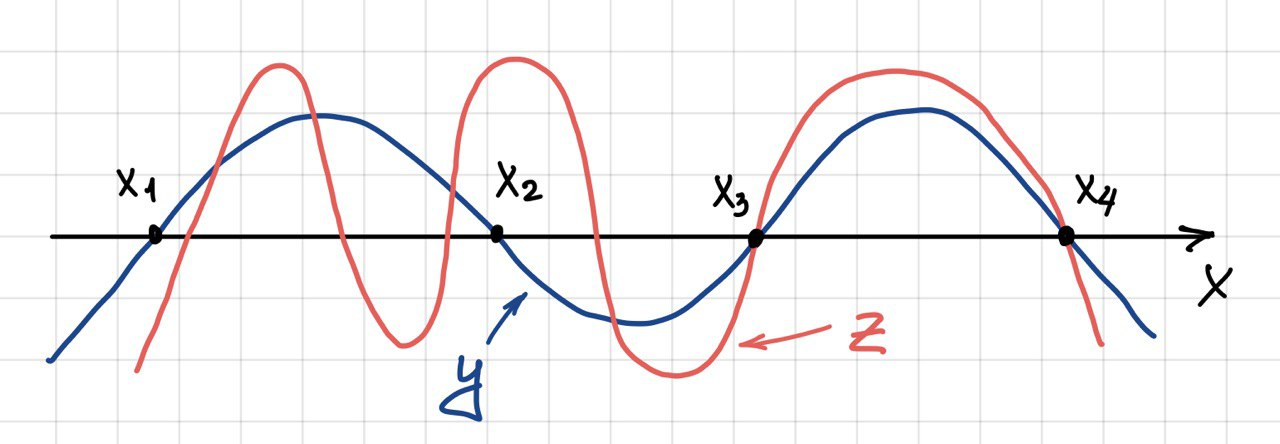
\includegraphics[width=1\linewidth]{images/shturma.jpg}
\end{center}
    \end{minipage}
\end{figure}
\\
\Proof Будем действовать от противного: предположим, что $z(x) \neq 0$ на $(x_1, x_2)$, т.е. например, $z(x) > 0$.
\newline Без потери общности предположим, что $y(x) > 0$ на $(x_1,x_2)$. Из условия теоремы: $y(x_1)=y(x_2)=0$. Тогда
\begin{equation*}
    y'(x_1)=\lim\limits_{x\to x_1+0}\frac{y(x)-y(x_1)}{x-x_1}\geqslant 0
    \qquad \qquad y'(x_2)=\lim\limits_{x\to x_2-0}\frac{y(x)-y(x_2)}{x-x_2}\leqslant 0
\end{equation*}
Но поскольку $x_1,x_2$ -- простые нули (т.к. решения нетривиальные), то $y'(x_1)>0$ и $y'(x_2)<0$.
\\
Посчитаем $(3)\cdot z - (4) \cdot y$:
\setcounter{equation}{4}
\begin{equation}\label{prom}
    y''z - z''y = (Q-q)yz
\end{equation}
Вычислим интеграл левой части:
\begin{align*}
    \int\limits_{x_1}^{x_2}(y''z-z''y)dx &= \int\limits_{x_1}^{x_2}zdy' - \int\limits_{x_1}^{x_2}ydz' = \\ &=
    (zy')\Big|_{x_1}^{x_2}-\int\limits_{x_1}^{x_2}y'dz \;-\; (yz')\Big|_{x_1}^{x_2} + \int\limits_{x_1}^{x_2}z'dy = 
\end{align*}
При этом верно: $dz=z'dx$ и $dy=y'dx$. Поэтому полученные интегралы совпадают и сокращаются. 
\begin{align*}
    = (zy')\Big|_{x_1}^{x_2} - \cancelto{0}{(yz')\Big|_{x_1}^{x_2}} \text{\qquad сокращается, так как $y(x_1)=y(x_2)=0$}
\end{align*}
Тогда (\ref{prom}) принимает вид:
\begin{equation}\label{final}
    z(x_2)y'(x_2)-z(x_1)y'(x_1) = \int\limits_{x_1}^{x_2}\underbrace{(Q-q)yz}_{\geqslant0}\,dx \geqslant 0
\end{equation}
Далее возможны следующие варианты:
\begin{equation*}
    \text{$\bullet$ \;$z > 0$ на $[x_1, x_2]$ \qquad\; $\bullet$ \;$z > 0$ на $[x_1, x_2)$, и $z(x_2) = 0$ \qquad\; $\bullet$\; $z > 0$ на $(x_1, x_2]$, и $z(x_1) = 0$ }
\end{equation*}
Заметим, что левая часть (\ref{final}) во всех случаях отрицательна $\Rightarrow$ противоречие.\; \EndProof
\bigbreak
\noindent \textbf{Следствие 1:} Если $q(x) \leqslant 0$, то любое нетривиальное решение уравнения $y''+q(x)y = 0$ имеет не более одного нуля.
\\
\Proof Предположим, что есть нетривиальное решение $y(x)$, у которого есть 2 последовательных нуля.
\\
Тогда пусть $Q(x)\equiv0$, то есть $z''+0\cdot z = 0 \;\; \Rightarrow \;\; z = ax + b \neq 0$. \newline Возьмем $z\equiv 5$. Но эта функция не имеет ни одного нуля $\;\Rightarrow\;$ противоречие с теоремой Штурма. \;\EndProof
\bigbreak
\noindent \textbf{Следствие 2:} Пусть $y_1(x)$ и $y_2(x)$ — линейно независимые решения уравнения $y'' +q(x) y = 0$. \newlineЕсли $x_1$ и $x_2$ — последовательные нули $y_1$, то между ними имеется ровно один
нуль $y_2$.
\\
\Proof Положим $q(x) \equiv Q(x)$. Заметим, что $y_1$ и $y_2$ не обращаются одновременно в нуль в $x_1$ и $x_2$ (ввиду линейной независимости). Если предположить, что между
$x_1$ и $x_2$ лежит \underline{хотя бы два} нуля $y_2$, то аналогичным образом получается, что между этими нулями есть ещё хотя бы один нуль $y_1$. \; \EndProof
\bigbreak
\noindent \textbf{Следствие 3:} Если некоторое нетривиальное решение уравнения $y'' + q(x) y = 0$ имеет
бесконечно много нулей, то и любое другое решение также имеет бесконечно много нулей.
\newpage

\subsection{Уравнения Бесселя и некоторые свойства его решений}
\noindent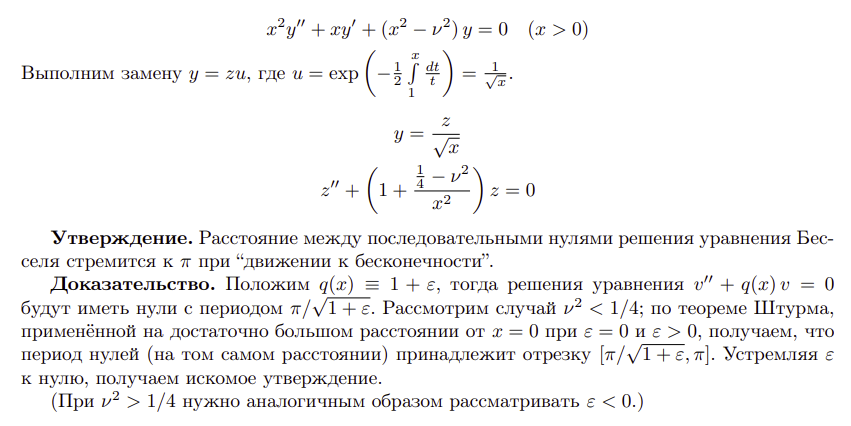
\includegraphics[width=0.95\linewidth]{images/bess.png}

\subsubsection*{Решения}
Доказано, что в общем случае решения уравнения Бесселя не выражаются через композиции коэффициентов уравнения, элементарных функций и их интегралов. Однако эти
решения можно выразить как степенные ряды.

\textbf{Функция Бесселя первого рода}
\begin{equation*}
    J_\nu(x) = \sum\limits_{k=0}^{\infty}{\frac{(-1)^k\Big(\frac{x}{2}\Big)^{2k+\nu}}{\Gamma(k + 1)\Gamma(k+1+\nu)}}
\end{equation*}
где $\Gamma$ -- это гамма-функция: $\Gamma(k+1) = k!$ \;и\; $\Gamma(k+1+\alpha) = (\alpha+1)\ldots(\alpha+k)\Gamma(\alpha+1)$

\subsubsection*{Cвойство решения:}
\begin{center}
    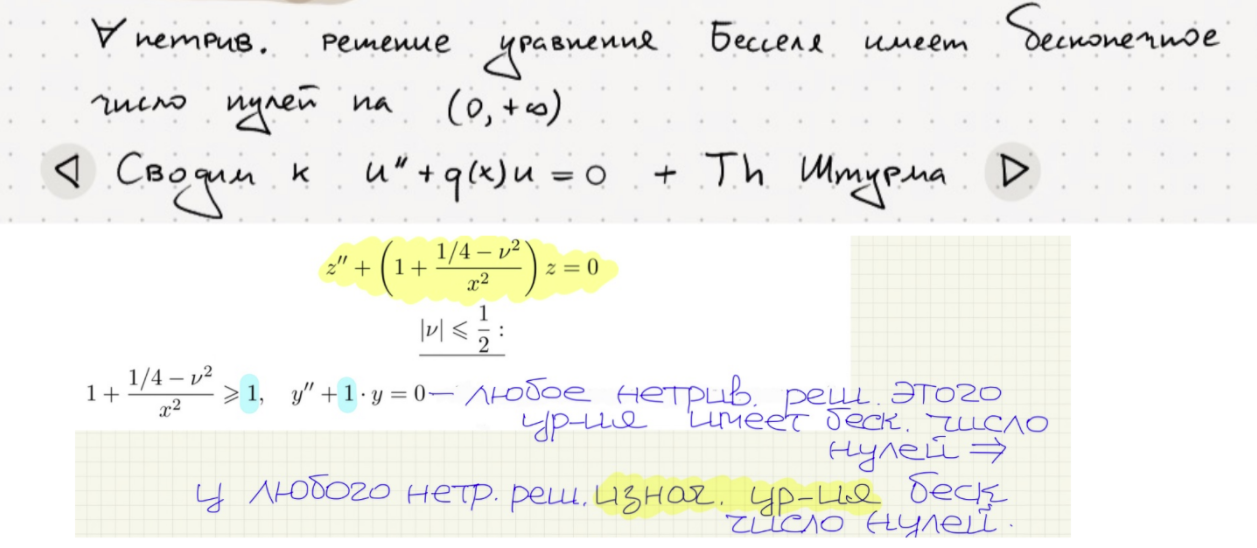
\includegraphics[width=0.95\linewidth]{images/bess_1.png}
\end{center}
\begin{center}
    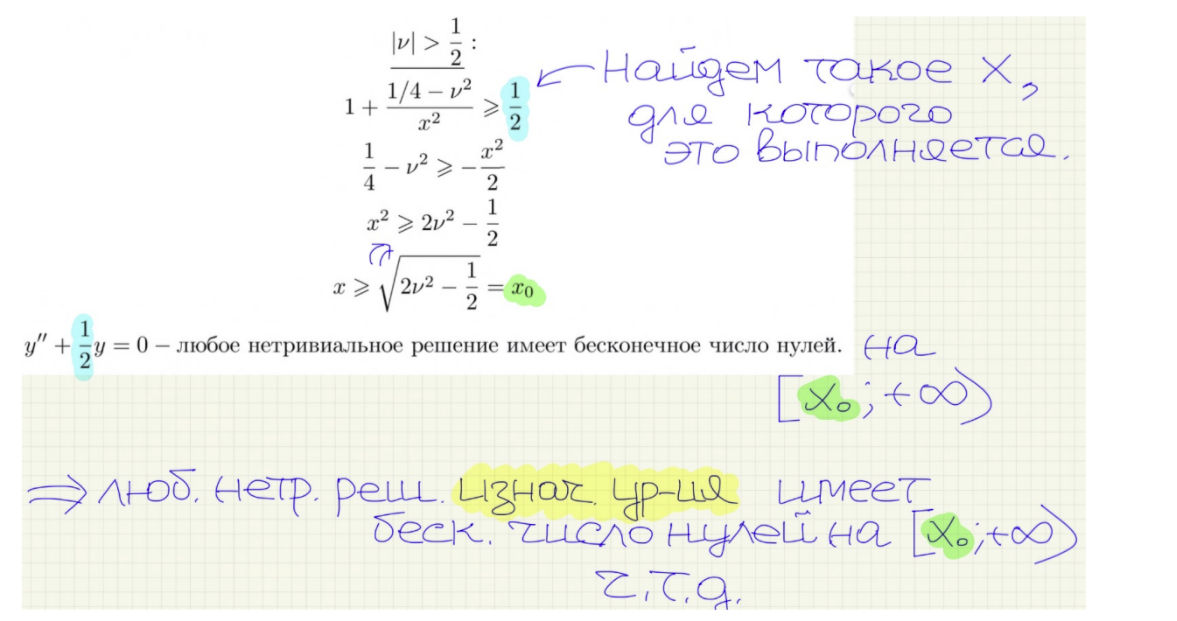
\includegraphics[width=0.95\linewidth]{images/bess_2.png}
\end{center}
\newpage

\section{Автономные системы дифференциальных уравнений}

\subsection{Основные понятия. Свойства решений и фазовых траекторий}
\setcounter{equation}{0}
Нормальной автономной системой дифференциальных уравнений порядка $n$ называется система
\begin{equation}\label{autonom-sys}
    \dot{x}(t) = f(x)
\end{equation}
где $f(x)$— заданная действительная вектор-функция c $n$ компонентами определенная в некоторой области (называется фазовым пространством автономной системы) $\Omega$ евклидового пространства $\mathbb{R}_x^n$ с
фиксированной прямоугольной декартовой системой координат $x_1, \ldots, x_n$.

В системе~(\ref{autonom-sys}) $t$~--- независимая переменная, которую принято называть временем и считать лежащей в $\mathbb{R}_t^1$, а $x(t)$~--- неизвестная действительная вектор-функция c $n$ компонентами.

В дальнейшем будем предполагать, что $f(x)$ удовлетворяет в области $\Omega$ условию Липшица. Это гарантирует существование и единственность непродолжимого решения системы~(\ref{autonom-sys}) при начальном условии
\begin{equation}\label{autonom-sys-condition}
    x(t_0) = x_0, x_0 \in \Omega,
\end{equation}
на некотором промежутке $I = I(t_0, x_0)$ оси $t$, содержащей точку $t_0$.

Произвольная нормальная система дифференциальных уравнений
\begin{equation}\label{autonom-sys-custom}
    \dot{x}(t) = f(x, t)
\end{equation}
всегда сводится к автономной системе путем увеличения числа неизвестных функций на единицу. Если положить \(t = x_{n + 1}\), то получаем автономную систему с \((n - 1)\) неизвестными функциями:
\[
 \begin{cases}
 \dot{x}(t) = f(x, x_{n + 1})\\
 \dot{x}_{n+1} = 1
 \end{cases}.
\]

Таким образом, автономная система~(\ref{autonom-sys}) отличается от любой системы~(\ref{autonom-sys-custom}) тем, что правая часть~(\ref{autonom-sys}) не содержит переменной $t$.

\begin{definition}
Если \(x = \varphi(t)\)~--- решение системы~(\ref{autonom-sys}) на промежутке \(I \subseteq \mathbb{R}_t^1\), то оно определяет параметрически заданную кривую в области $\Omega$, т.е. множество точек \(\{\varphi(t)\} \in \Omega\) при всех \(t \in I\). Эта кривая в $\Omega$ называется фазовой траекторией автономной системы~(\ref{autonom-sys}).
\end{definition}

Интегральные кривые~(\ref{autonom-sys}) представляют собой графики решений \(x = \varphi(t)\) системы~(\ref{autonom-sys}) в бесконечном цилиндре
\[G = \{(x, t) \in \mathbb{R}_{(x, t)}^{n + 1} : x \in \Omega, t \in \mathbb{R}_t^1\}\]
\((n + 1)\)\,-мерного пространства $\mathbb{R}_{(x, t)}^{n + 1}$. 

Следовательно, фазовая траектория~(\ref{autonom-sys}) является проекцией интегральной кривой~(\ref{autonom-sys}) параллельно оси $t$ (см. рис.\,\ref{fkng-cylinder}). На траектории стрелкой указывают ее ориентацию, т.е. направление движения по ней в сторону возрастания $t$.

\begin{figure}[ht]\label{fkng-cylinder}
    \centering
    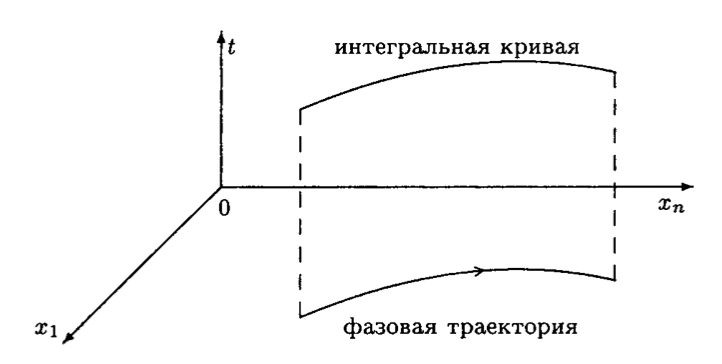
\includegraphics[scale=0.8]{sections/Sasha/images/fkng-cylinder.png}
    \caption{Цилиндр о котором речь}
\end{figure}

Из теоремы существования и единственности решения задачи Коши~(\ref{autonom-sys}),~(\ref{autonom-sys-condition}) получаем, что через каждую точку \(x_0 \in \Omega\) проходит единственная траектория~(\ref{autonom-sys}), определенная в некоторой окрестности $t_0$. При некоторых
достаточных условиях эта траектория определена при всех \(t \in \mathbb{R}_t^1\).

\paragraph{Свойства фазовых траекторий}

\begin{theorem}[очев]
Если \(x(t) = \varphi(t)\)~--- решение~(\ref{autonom-sys}) при \(t \in (\alpha ; \beta)\) и $C$~--- некоторое действительное число, то \(x(t) = \varphi(t + c)\)~--- решение при \(t \in (\alpha - c; \beta - c)\).
\end{theorem}
\begin{center}
    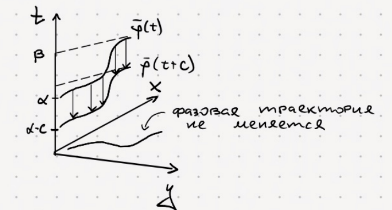
\includegraphics[width=0.5\linewidth]{images/proof.png}
\end{center}

\begin{theorem}
Если две фазовых траектории \(x(t) = \varphi(t), t \in I_1\) и \(x(t) = \psi(t), t \in I_2\)~--- решения~(\ref{autonom-sys}) и \[x_0 = \varphi(t_1) = \psi(t_2)\], то \(\psi(t) \equiv \varphi(t + t_1 - t_2)\) для всех $t$ для которых определены обе части тождества
\end{theorem}
\begin{proof}
Рассмотрим \(y = \varphi_1(t) = \varphi(t + t_1 - t_2), t + t_1 - t_2 \in I_1\), тогда
\( \varphi_1(t_2) = \varphi(t_1) = \psi(t_2)\). Из этого следует, что \(\varphi_1(t_2) =\psi(t_2) = x_0\). Но тогда по теореме существования и единственности, для всех $t$ для которых определены обе части тождества, получаем необходимое тождество.
\end{proof}

\begin{definition}
Решение системы~(\ref{autonom-sys}) \(x(t) = \varphi(t) \equiv x_0 \in \Omega, \forall t \in \mathbb{R}_t^1\) называется положением равновесия или точкой покоя системы~(\ref{autonom-sys})
\end{definition}

\begin{theorem}
Точка \(x_0 \in \Omega \) является положением равновесия системы~(\ref{autonom-sys}) тогда и только тогда когда \(f(x_0) = 0\).
\end{theorem}
\begin{proof}
\fbox{$\Longrightarrow$} Пусть \(x = x_0\)~--- п.р.~(\ref{autonom-sys}). Тогда \(\dot{x} = f(x_0) = 0\).\\
\fbox{$\Longleftarrow$} Пусть \(f(x_0) = 0\). Тогда \(\dot{x} = 0\) и \(x = x_0\).
\end{proof}

\begin{definition}
Если решение системы~(\ref{autonom-sys}) \(x = \varphi(t), \forall t \in \mathbb{R} _t^1\) и является периодической вектор-функцией с периодом $T$, то соответствующая ему фазовая траектория называется циклом системы.
\end{definition}

\begin{theorem}[б/д]
Все фазовые траектории системы~(\ref{autonom-sys}) принадлежат одному из трех классов:
\begin{enumerate}
    \item положение равновесия;
    \item замкнутая траектория (цикл);
    \item траектория без самопересечений.
\end{enumerate}
\end{theorem}
\begin{figure}[h]
    \begin{minipage}[h]{0.5\linewidth}
    Замкнутая траектория:
\begin{center}
    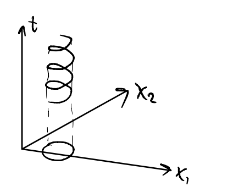
\includegraphics[width=0.5\linewidth]{images/cycle.png}
\end{center}
    \end{minipage}
    \hspace{-4ex}
    \begin{minipage}[h]{0.5\linewidth}
Иллюстрация к теореме 5.3:
\begin{center}
    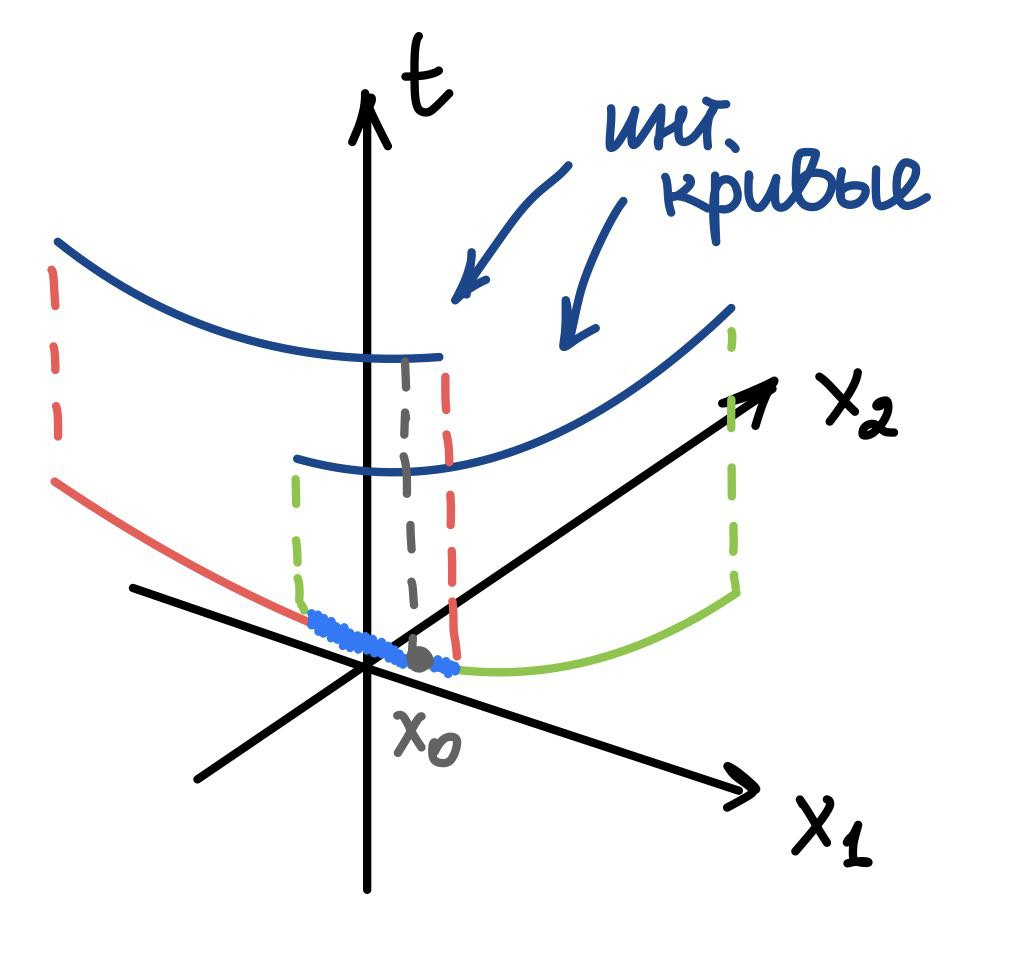
\includegraphics[width=0.5\linewidth]{images/th2.jpg}
\end{center}
    \end{minipage}
\end{figure}




\newpage

\subsection{Классификация положений равновесия линейной автономной системы второго порядка}
Линейная автономная система второго порядка записывается так:
\begin{equation}\label{autonom-sys-2d}
    \begin{cases}
    \dot{x_1} = a_{11} x_1 + a_{12} x_2 \\
    \dot{x_2} = a_{21} x_1 + a_{22} x_2
    \end{cases}
\end{equation}

Также удобно обозначить \(x = x_1, y = x_2\). Числа \(a_{11}, a_{12}, a_{21}, a_{22}\)~--- заданные действительные числа, \(t \in R_t^1\). Введем матрицу 
\[A = \begin{pmatrix} a_{11} & a_{12} \\ a_{21} & a_{22}\end{pmatrix}.\]

\begin{definition}
Линейная автономная система~(\ref{autonom-sys-2d}) называется простой, если матрица $A$ — невырожденна. В противном случае система~(\ref{autonom-sys-2d}) называется сложной.
\end{definition}

\begin{lemmanote}
Если задано автономное уравнение второго порядка
\begin{equation}
    \ddot{x} + a \dot{x} + b x = 0
\end{equation}
с действительными коэфициентами $a, b$, то его положениями равновесия называются положения равновесия автономной системы вида
\begin{equation}
\begin{cases}
\dot{x} = y\\
\dot{y} = -bx - ay.
\end{cases}
\end{equation}
\end{lemmanote}

Рассмотрим различные случаи. Далее, $\lambda_1, \lambda_2$~--- собственные значения матрицы $A$, a $h_1, h_2$~--- соответсвтующие собственные векторы. 

\paragraph{Случай простой системы}

\begin{enumerate}
    \item Случай действительных $\lambda_1, \lambda_2$.\\
        Если они различны, то существует базис из собственных векторов. Все действительные решения задаются формулой
        \[x(t) = c_1 e^{\lambda_1 t} h_1 + c_2 e^{\lambda_2 t} h_2.\] В базисе из собственных векторов координаты решения \(x(t)\) системы~(\ref{autonom-sys-2d}) имеют вид
        \[\zeta_1 = c_1 e^{\lambda_1 t},\;\; \zeta_2 =  c_2 e^{\lambda_2 t}.\] В силу симметрии, достаточно исследовать систему при $\zeta_1 > 0, \zeta_2 > 0.$
        \begin{enumerate}
        \item Пусть $\lambda_1$ < 0, $\lambda_2$ < 0 и $|\lambda_1| < |\lambda_2|$.\\
        Тогда:
        \begin{itemize}
        \item $c_1 = c_2 = 0$ дает положение равновесия $x = 0$;
        \item $c_1 >0, c_2 = 0$ дает полуось $\zeta_1 > 0$, причем $\zeta_1 \longrightarrow +0, t \longrightarrow +\infty$;
        \item $c_1 = 0, c_2 > 0$ дает полуось $\zeta_2 > 0$, причем $\zeta_2 \longrightarrow +0, t \longrightarrow +\infty$;
        \item $c_1 > 0, c_2 > 0$, то 
        \[e^t = \Big(\frac{\zeta_1}{c_1}\Big)^{\frac{1}{\lambda_1}} \;\; \Rightarrow \;\; \zeta_2 = c \zeta_1^{\alpha}, \quad c = c_2 \cdot c_1^{-\frac{\lambda_2}{\lambda_1}}, \quad \alpha = \frac{\lambda_2}{\lambda_1} > 1.\]
        В этом случае траектории являются кривыми типа ветвей параболы, касающихся в пределе при $t \longrightarrow +\infty$ оси $\zeta_1$ в начале координат.
        \end{itemize}
        В целом в случае (a) получаем семейство фазовых траекторий типа ветвей параболы и пять специальных траекторий: положение равновесия $x = 0$ и четыре полуоси осей координат $\zeta_1, \zeta_2$. Схематически фазовый портрет системы~(\ref{autonom-sys-2d}) в случае (a) показан на рисунке ниже.\\
        Стрелка на траектории показывает направление движения при $t \longrightarrow +\infty$.
        В этом случае положение равновесия $x = 0$ называется \textbf{устойчивым узлом} системы~(\ref{autonom-sys-2d}).
        
    \item Пусть $\lambda_1$ > 0, $\lambda_2$ > 0 и $|\lambda_1| < |\lambda_2|$.\\
        Меняется лишь направление движения по траекториям. В данном случае положение равновесия называется \textbf{неустойчивым узлом}. Схематически фазовый портрет системы~(\ref{autonom-sys-2d}) в случае (b) показан на рисунке ниже.
        \begin{figure}[H]\label{autonom-casea}
            \centering
            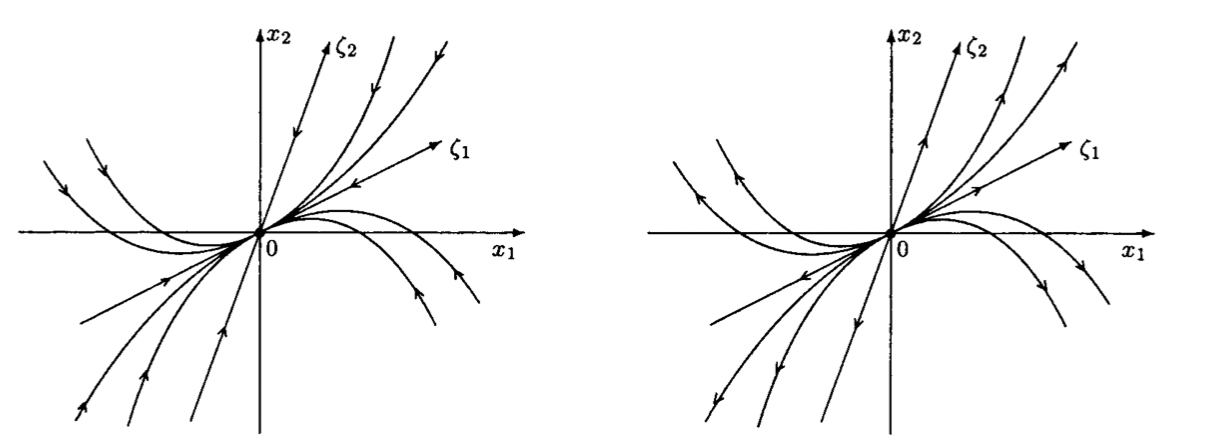
\includegraphics[scale=0.8]{sections/Sasha/images/autonom-casea.png}
            \caption{Слева $\lambda_1$ < 0, $\lambda_2$ < 0 и $|\lambda_1| < |\lambda_2|$, справа $\lambda_1$ > 0, $\lambda_2$ > 0 и $|\lambda_1| < |\lambda_2|$}
        \end{figure}
        
    \item Пусть \(\lambda_1 < 0 < \lambda_2\).\\
        Тогда 
        \begin{itemize}
        \item $c_1 = c_2 = 0$ дает положение равновесия $x = 0$;
        \item $c_1 >0, c_2 = 0$ дает полуось $\zeta_1 > 0$, причем $\zeta_1 \longrightarrow +0, t \longrightarrow +\infty$;
        \item $c_1 = 0, c_2 > 0$ дает полуось $\zeta_2 > 0$, причем $\zeta_2 \longrightarrow +\infty, t \longrightarrow +\infty$;
        \item $c_1 > 0, c_2 > 0$, то как и в случае (a):
        \[\zeta_2 = c \zeta_1^{\alpha}, \;\; c = c_2 \cdot c_1^{-\frac{\lambda_2}{\lambda_1}}, \;\; \alpha = \frac{\lambda_2}{\lambda_1} < 0.\]
        В этом случае траектории являются кривыми типа гипербол.
        \end{itemize}
        В целом в случае (с) получаем семейство фазовых траекторий типа гипербол и пять специальных траекторий: положение равновесия $x = 0$ и четыре полуоси осей координат $\zeta_1, \zeta_2$. Эти полуоси служат асимптотами для гипербол и называются сепаратисами.\\
        Положение равновесия $x = 0$ системы~(\ref{autonom-sys-2d}) в случае (c) \textbf{называется седлом}. Схематически фазовый портрет системы~(\ref{autonom-sys-2d}) в случае (c) показан на рисунке ниже.
        \begin{figure}[H]\label{autonom-casec}
            \centering
            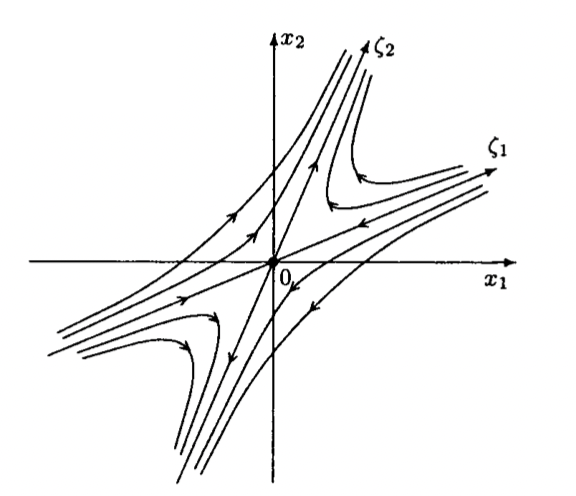
\includegraphics[scale=0.8]{sections/Sasha/images/autonom-casec.png}
            \caption{$\lambda_1 < 0 < \lambda_2$}
        \end{figure}
    
    \item Пусть \(\lambda_1 = \lambda_2 = \lambda\) и существует базис плоскости из собственных векторов $h_1, h_2$.
        Все действительные решения задаются формулой
        \[x(t) = e^{\lambda t} ( c_1 h_1 + c_2 h_2).\]
        \[\frac{dx_1}{dx_2}=\frac{c_1h_{11} + c_2h_{12}}{c_1h_{21} + c_2h_{22}} \text{ -- не зависит от } t\]
        Поэтому каждое такое решение описывает луч, выходящий из начала координат, причем движение по лучу при \(t \longrightarrow +\infty\) идет к нулю при \(\lambda < 0\) и от нуля при \(\lambda > 0\).\\
        При \(\lambda < 0\) положение равновесия $x = 0$ называется \textbf{устойчивым дикритическим узлом}, а при \(\lambda > 0\) \textbf{неустойчивым дикритическим узлом}. Схематически данный случай изображен на рисунке ниже.
        \begin{figure}[H]\label{autonom-cased}
            \centering
            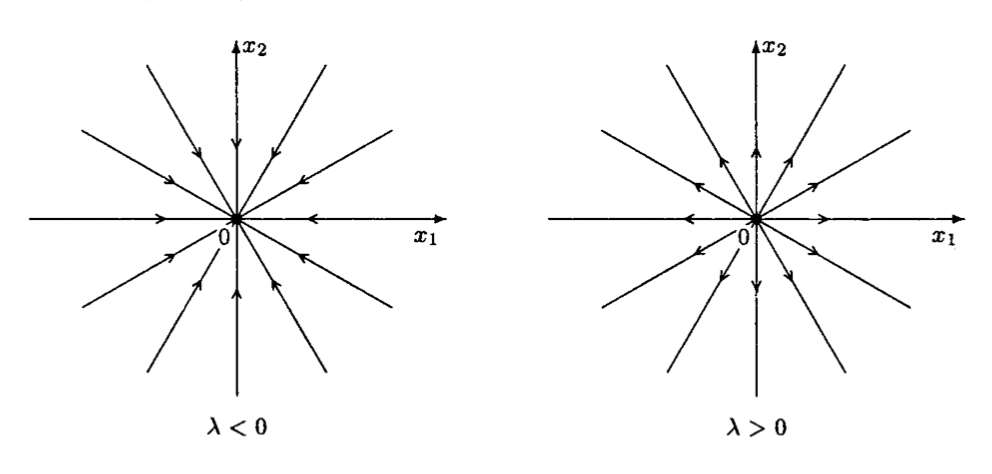
\includegraphics[scale=0.8]{sections/Sasha/images/autonom-cased.png}
            \caption{Дикритические узлы}
        \end{figure}

     \item Пусть \(\lambda_1 = \lambda_2 = \lambda\) и существует базис плоскости из собственного вектора $h_1$ и присоединенного к нему $h_{12}$.
        Все действительные решения задаются формулой
        \[x(t) = c_1 e^{\lambda t} h_1 + c_2 e^{\lambda t} (h_{12} + t h_1).\]
        В базисе из собственных векторов координаты решения \(x(t)\) системы~(\ref{autonom-sys-2d}) имеют вид
        \[\zeta_1 = (c_1 + c_2 t) e^{\lambda t}, \;\; \zeta_2 =  c_2 e^{\lambda t}.\]
        Для \(\lambda < 0\) получаем:
        \begin{itemize}
            \item при \(c_1 = c_2 = 0\) положение равновесия \(x = 0\);
            \item при \(c_1 \neq 0, c_2 = 0\) две полуоси \(\zeta_1 < 0, \zeta_1 > 0\) причем при \(t \longrightarrow +\infty\) идет к нулю; (т.е. получаем прямую $\zeta_1$).
            \item при \(c_2 \neq 0\) выносим t за скобки:
            \[x(t) = t\Big(c_2h_1e^{\lambda t} + \frac{1}{t}(c_1h_1e^{\lambda t} + c_2h_{2}e^{\lambda t})\Big) = \big(tc_2h_1+o(1)\big)e^{\lambda t} \text{ , где $o(1) \stackrel{t\to\infty}{\longrightarrow} 0$.}\]  Отсюда получаем, что $x(t)\; ||\; h_1$. При переходе в базис, в котором мы работали это значит $x(t)\; ||\; \zeta_1$. Множитель $t > 0$ при \(t \longrightarrow +\infty\) и $t < 0$ при \(t \longrightarrow -\infty\). Значит, траектория разворачивается в противоположном направлении. 
        \end{itemize}
        В случае \(\lambda < 0\) положение равновесия $x = 0$ называется \textbf{устойчивым вырожденным узлом} системы~(\ref{autonom-sys-2d}).
        
        В случае \(\lambda > 0\) траеткории получаются из описанных выше путем зеркального отображения относительно оси $\zeta_2$, а движение по ним при \(t \longrightarrow +\infty\) идет от начала координат.
        
        В случае \(\lambda > 0\) положение равновесия $x=0$ называется \textbf{неустойчивым вырожденным узлом}. Схематически фазовый портрет показан на рисунке ниже.
        \begin{figure}[H]\label{autonom-casee}
            \centering
            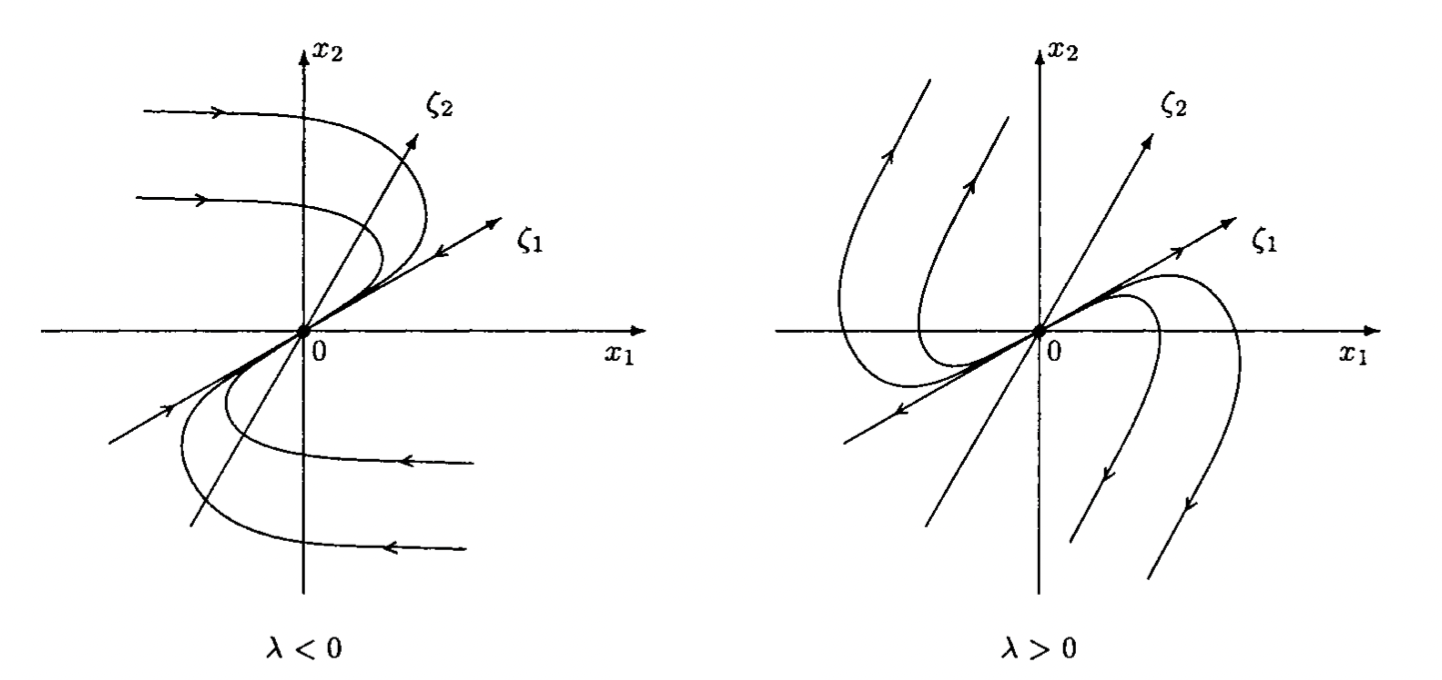
\includegraphics[scale=0.6]{sections/Sasha/images/autonom-casee.png}
            \caption{Вырожденные узлы}
        \end{figure}
    \end{enumerate}
    \item Случай комплексных $\lambda_1, \lambda_2$.\\
    Если \(\lambda_1 = \mu + i \nu\), где $\nu > 0$, то в силу действительности $A$ имеем \(\lambda_2 = \overline{\lambda_1} = \mu - i \nu\). Обозначим через \(h = h_1 - i h_2\) собственный вектор $A$ для $\lambda_1$, где $h_1, h_2$~--- действительные векторы. Тогда \(\overline{h} = h_1 + i h_2\) является собственным вектором для $\lambda_2$. Общее действительное решение~(\ref{autonom-sys-2d}) в этом случае имеет вид
    \[x(t) = c e^{\lambda_1 t}h + \overline{c} e^{\overline{\lambda_1}t} \overline{h},\]
    где $c$~--- произвольная комплексная константа.
    
    Если положить 
    \[c = |c|e^{i\varphi}, \varphi \in [0; 2\pi),\]
    то \(\overline{c} = |c| e^{-i\varphi}\) и общее решение преобразуется к виду \[x(t) = 2 |c|e^{\mu t}[\cos{(\varphi + \nu t)} h_1 + \sin{(\varphi + \nu t)} h_2].\]
    Так как $h_1$ и $h_2$~--- линейно независимы, то взяв их в качестве нового базиса плоскости координаты решения в этом базисе будут иметь вид
    \[\zeta_1(t) = 2 |c|e^{\mu t} cos(\varphi + \nu t), \;\; \zeta_2(t) = 2 |c|e^{\mu t}sin(\varphi + \nu t).\]
    Положив \(r(t) = 2 |c| e^{\nu t}, \psi(t) = \varphi + \nu t\), отсюда получаем уравнение траекторий в полярных координатах $r, \psi$
    \[r(t) = 2|c| \cdot \exp\Big(\mu \frac{\psi - \varphi}{\nu}\Big).\]
    
    При $c \neq 0, \mu \neq 0$ фазовые траектории представляют собой кривые типа логарифмических спиралей, а при $\mu = 0$~--- кривые типа эллипсов.
    \begin{enumerate}
    \item Пусть $\mu < 0$.\\
        Тогда при $c = 0$ получаем положение равновесия $x=0$, а при $c \neq 0$ фазовая точка по спирали \underline{движется} к $x=0$ при \(t \longrightarrow +\infty\) , так как $r(t) \longrightarrow +0, \psi(t) \longrightarrow +\infty$ при \(t \longrightarrow +\infty\).
        
        Направление закручивания определяется направлением фазовой скорости. Например, можно рассмотреть точку $(0, 1)$ и тогда $f(x)$ будет иметь компоненты $a_{12}, a_{22}$. Возможные два различных фазовых портрета в этом случае схематически показаны на рисунке ниже
        \begin{figure}[H]\label{autonom-compla}
                \centering
                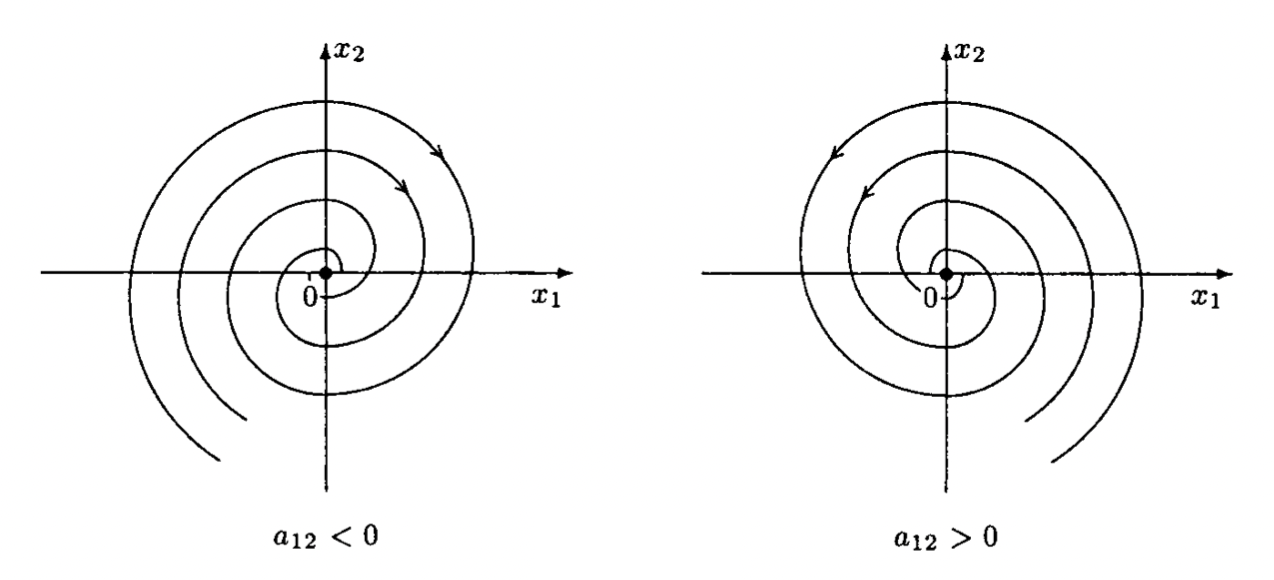
\includegraphics[scale=0.6]{sections/Sasha/images/autonom-compla.png}
                \caption{}
        \end{figure}
        Положение равновесия $x=0$ в этом случае называется \textbf{устойчиывым фокусом} системы.
    
    \item Пусть $\mu > 0$.\\
        Тогда при $c = 0$ получаем положение равновесия $x=0$, а при $c \neq 0$ фазовая точка по спирали \underline{удаляется от} $x=0$ при \(t \longrightarrow +\infty\), так как $r(t) \longrightarrow +\infty, \psi(t) \longrightarrow +\infty$ при \(t \longrightarrow +\infty\).
        
        В этом случае положение равновесия $x=0$ называется \textbf{неустойчивым фокусом} системы. Возможные в этом случае два различных фазовых портрета схематически показаны на рисунке ниже.
        \begin{figure}[H]\label{autonom-complb}
                \centering
                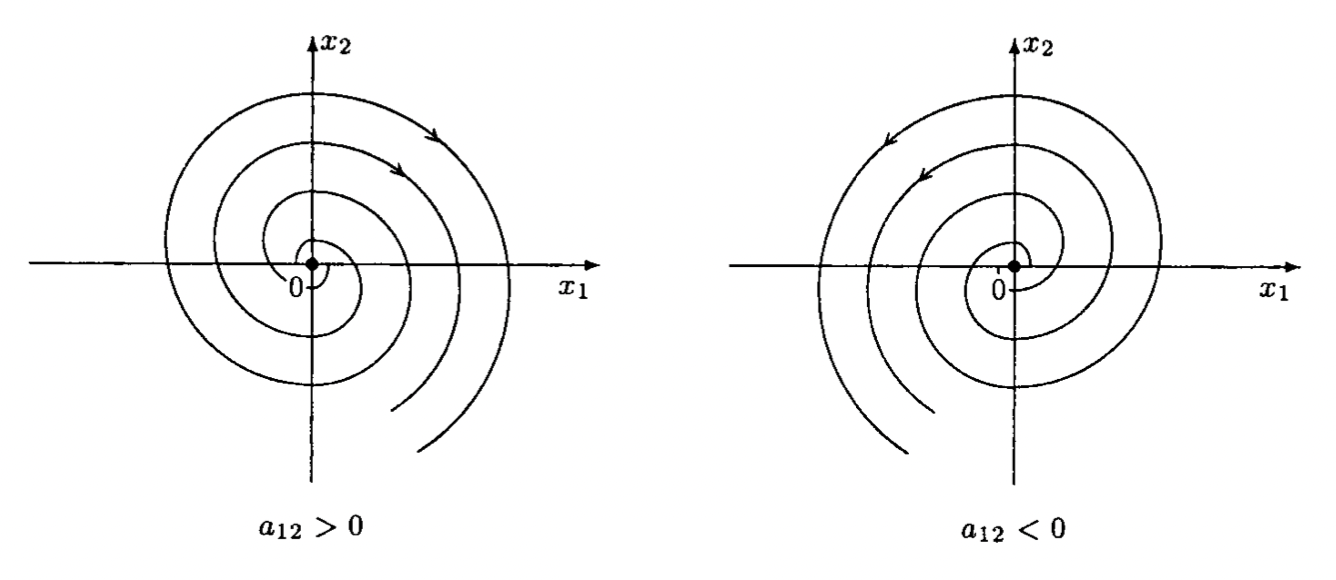
\includegraphics[scale=0.6]{sections/Sasha/images/autonom-complb.png}
                \caption{}
        \end{figure}
    \item Пусть $\mu = 0$.\\
        Тогда в произвольном базисе $h_1$ и $h_2$ при $c \neq 0$ траектории — кривые типа эллипса, а при $c = 0$~--- положение равновесия $x=0$. В этом случае положение равновесия называется \textbf{центром для системы}~(\ref{autonom-sys-2d}). В зависимости от направления обхода эллипсов возможные фазовые портреты схематиески изображены на рисунке ниже.
        \begin{figure}[H]\label{autonom-complc}
            \centering
            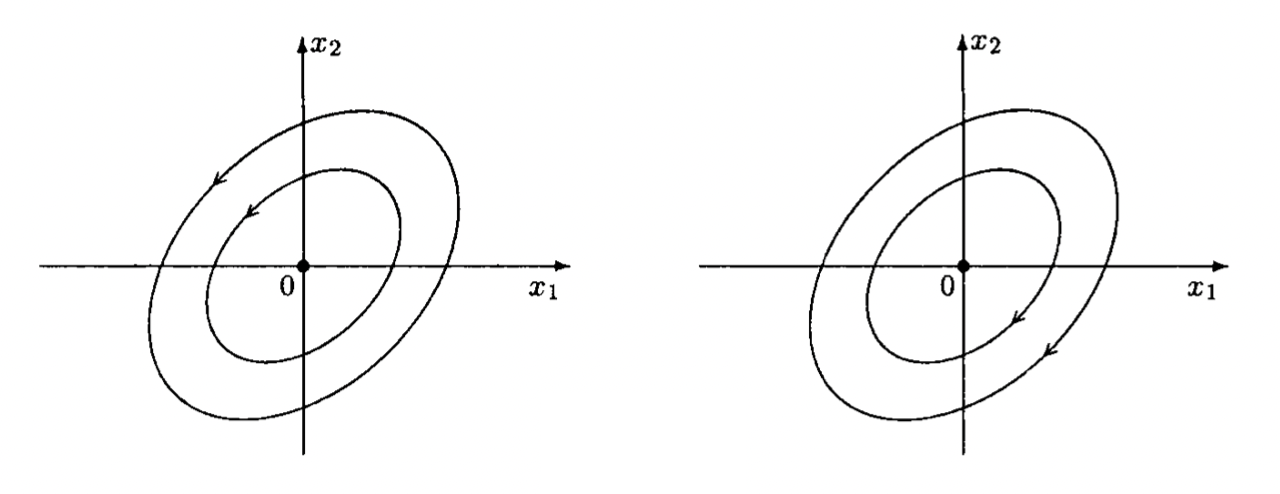
\includegraphics[scale=0.6]{sections/Sasha/images/autonom-complc.png}
            \caption{}
        \end{figure}
    \end{enumerate}
\end{enumerate}

Таким образом, для простой линейной автономной системы существует всего (хах, "всего") тринадцать различных фазовых портретов.

\paragraph{Случай сложной системы}
Напомню, что система~(\ref{autonom-sys-2d}) называется сложной если матрица $A$ вырождена.

\begin{enumerate}[label=(\alph*)]
    \item Пусть $\lambda_1 \neq 0, \lambda_2 = 0$.\\
        Тогда \(\zeta_1(t) = c_1 e^{\lambda_1 t}, \;\zeta_2(t) = c_2\). Отсюда ясно, что все точки прямой $\zeta_1= 0$ являются положениями равновесия и что оба луча луча каждой прямой $\zeta_2(t) = c_2$ являются траекториями~(\ref{autonom-sys-2d}).
        
        В зависимости от знака $\lambda_1$ движенеи по ним при \(t \longrightarrow +\infty\) идет либо к прямой $\zeta_1= 0$ либо от нее. В зависимости от знака $\lambda_1$ возможны два схематически представленных на рисунке ниже
        \begin{figure}[H]\label{autonom-triviala}
            \centering
            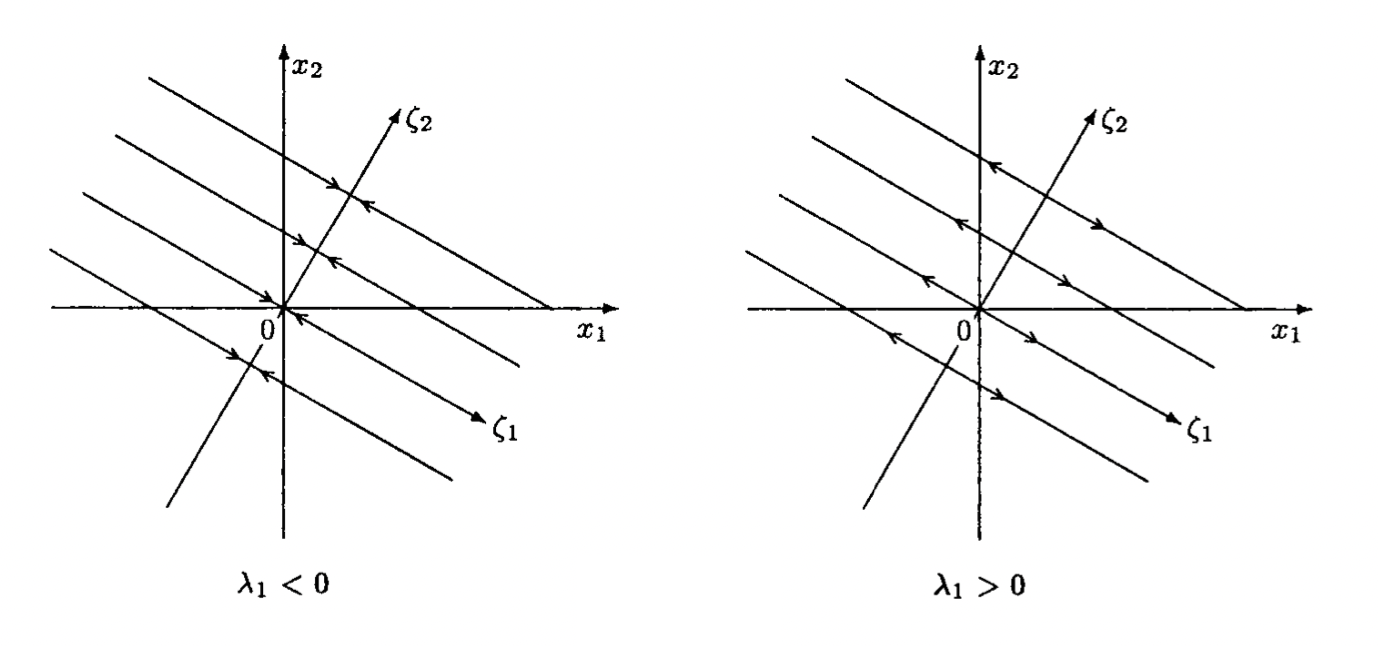
\includegraphics[scale=0.6]{sections/Sasha/images/autonom-triviala.png}
            \caption{}
        \end{figure}
        
    \item Пусть $\lambda_1 = \lambda_2 = 0$.\\
        Если матрица $A$ нулевая,  то каждая точка плоскости является положением равновесия. 
        
        Если же $A$ ненулевая, то существует базис плоскости из собственного вектора $h_1$ и присоединенного к нему $h_2$. В этом базисе  решение имеет координаты 
        \[\zeta_1(t) = c_1 + c_2 t, \;\; \zeta_2(t) = c_2.\]
        Отсюда ясно, что все точки прямой $\zeta_2= 0$ являются положениями равновесия. Каждая из прямых $\zeta_2 = c$ является траекторией и при \(t \longrightarrow +\infty\) движение по ним идет слева направо при $\zeta_2>0$ и справа налево при $\zeta_2<0$. Изображено на рисунке ниже.
        \begin{figure}[H]\label{autonom-trivialb}
            \centering
            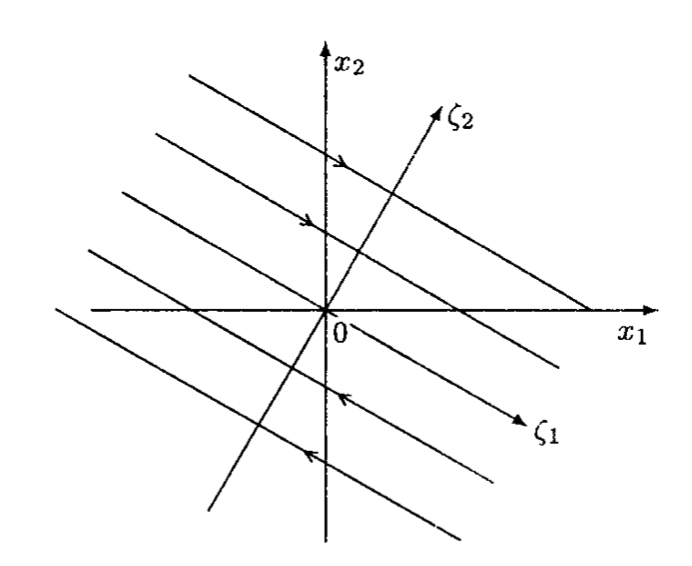
\includegraphics[scale=0.6]{sections/Sasha/images/autonom-trivialb.png}
            \caption{}
        \end{figure}
\end{enumerate}

Таким образом, для сложной линейной автономной системы существует всего четыре различных фазовых портрета.

\newpage

\subsection{Характер поведения фазовых траекторий в окрестности положения равновесия двумерной автономной нелинейной системы. Теорема о выпрямлении траекторий (б/д)}
\label{autonom-stratify}
Нелинейная автономная система задается

\begin{equation}\label{autonom-nonlin-sys}
    \begin{cases}
    \dot{x_1} = f_1(x_1, x_2)\\
    \dot{x_2} = f_2(x_1, x_2),
    \end{cases}
\end{equation}
где $f_1, f_2$~--- действительные дважды непрерывно дифференцируемые функции в некоторой области $\Omega$.

\begin{definition}
Две определенные на областях $\Omega_1$ и $\Omega_2$ системы будем называть качественно эквивалентными если существует взаимно однозначное и взаимно непрерывное отображение $F$ области $\Omega_1$ на $\Omega_2$, при котором каждая фазовая траектория первой системы с сохранением ориентации переходит в некую фазовую траекторию второй системы и наоборот. Если $F$ непрерывно дифференцируемо, то системы называются дифференцируемо эквивалентными.
\end{definition}

Пусть положение равновесия $x=0$. Разложим $f_1, f_2$ в окрестности положения равновесия по формуле Тейлора с остаточным членом в форме Пеано:
\begin{align*}
    f_1(x_1, x_2) = a_{11} x_1 + a_{12} x_2 + o(|x|),\\
    f_2(x_1, x_2) = a_{21} x_1 + a_{22} x_2 + o(|x|).
\end{align*}

Тогда, линейная однородная система 
\begin{equation}\label{autonom-nonlin-lin}
    \begin{cases}
    \dot{x_1} = a_{11} x_1 + a_{12} x_2\\
    \dot{x_2} = a_{21} x_1 + a_{22} x_2
    \end{cases}
\end{equation}
называется линеаризацией системы~(\ref{autonom-nonlin-sys}) в начале координат.

\begin{theorem}[О линеаризации (б/д)]
Если линеаризация~(\ref{autonom-nonlin-lin}) нелинейной системы~(\ref{autonom-nonlin-sys}) в начале координат $x=0$ является простой автономной системой и $x=0$ не является центром для системы~(\ref{autonom-nonlin-lin}), то в окрестности $x=0$ нелинейная система и ее линеаризация качественно эквивалентны.
\end{theorem}
Другими словами, если собственные значения матрицы линеаризации при $x=0$ имеют действительную часть отличную от нуля, то фазовый портрет~(\ref{autonom-nonlin-lin}) в окрестности $x=0$  получается из фазового портрета~(\ref{autonom-nonlin-sys}) небольшим искривлением.

\begin{theorem}[О выпрямлении траекторий (б/д)]
Пусть $f(x)$~--- непрерывно дифференцируемая вектор-функция в области $\Omega$ и пусть точка $a \in \Omega$ является обыкновенной точкой системы~(\ref{autonom-sys})~--- не точка равновесия. Тогда найдутся окрестность $\Omega_a$ точки $a$ и такая гладкая обратимая замена переменных в $\Omega_a$, что в окрестности $\Omega_a$ система~(\ref{autonom-sys}) примет вид 
\[
\dot{y_i} = 0,\;\; i = \overline{1, n-1},\;\; \dot{y_n} = 1,
\]
а траектории системы~(\ref{autonom-sys}) в окрестности $\Omega_a$ перейдут в отрезки прямых 
\[
y_i = c_i,\;\; i = \overline{1, n-1},\;\; y_n = t + c_n,
\]
где \(c_1, \ldots, c_n\)~--- постоянные.
\end{theorem}
\newpage

\subsection{Устойчивость по Ляпунову и асимптотическая устойчивость положения равновесия автономной системы. Достаточные условия асимптотической устойчивости положения равновесия линейной системы}
\setcounter{equation}{0}

Пусть задана автономная система 
\begin{equation}\label{autonomlap-sys}
    \dot{x}(t) = f(x), 
\end{equation}
где $t \in \mathbb{R}^1_x$ и $f(x)$~--- заданная непрерывно дифференцируемая вектор-функция с $n$ компонентами в некоторой области $\Omega$.

Зададим начальное условие 
\begin{equation}\label{autonomlap-sys-ny}
    x(0) = x_0 \in \Omega
\end{equation}
и обозначим решение задачи Коши~(\ref{autonomlap-sys}),~(\ref{autonomlap-sys-ny}) через $x(t, x_0)$. Пусть $a \in \Omega$ является положением равновесия~(\ref{autonomlap-sys}). Будем считать, что $a = 0$, в противном случае простой заменой сводится к этому случаю.

В дальнейшем считаем, что $\exists r > 0$ такое, что при $\forall x \in \Omega, |x_0| < r$, решение $x(t, x_0)$ определено для всех $t > 0$.

\begin{definition}[Устойчивость по Ляпунову]
Положение равновесия $x = 0$ автономной системы~(\ref{autonomlap-sys}) называется устойчивым по Ляпунову, если 
\[
\forall \varepsilon > 0 \;\; \exists \; 0 < \delta = \delta(\varepsilon) < r \;\;\left(\forall |x_0| < \delta \implies |x(t, x_0)| < \varepsilon \right)
\]
для всех $t > 0$.
В противном случае положение равновесия называется неустойчивым положением равновесия системы~(\ref{autonomlap-sys}).
\end{definition}

То есть, любая траектория~(\ref{autonomlap-sys}), начинающаяся в $\delta(\varepsilon)$ окрестности точки $O$, остается в наперед заданной $\varepsilon$~-окрестности точки $O$ при всех $t > 0$.

\begin{definition}[Асимптотическая устойчивость]
Устойчивое по Ляпунову положение равновесия $x = 0$ системы~(\ref{autonomlap-sys}) называется асимптотически устойчивым, если
\[
\exists r_1 \;\; \left(0 < r_1 \leq r,\; \lim_{t \rightarrow +\infty}x(t, x_0) = 0\right)
\]
при $|x_0| < r_1$.
\end{definition}

Асимптотическая устойчивость $x = 0$ геометрически означает, что любая траектория~(\ref{autonomlap-sys}), начинающаяся в некоторой окрестности $x = 0$ при $t \rightarrow +\infty$ стремится к $x = 0$. (Пример: неваляшка)

Исследуем устойчивость положения $x = 0$ для автономной линейной однородной системы с постоянными коэффициентами.
\begin{equation}\label{autonomlap-sys-const}
    \dot{x(t)} = Ax(t)
\end{equation}
\\
\Note За действительную часть числа обозначим $Re(\lambda) = \Re(\lambda)$

\begin{theorem}\label{autonomlap-th1}
Если $\Re(\lambda_k) < 0$ для всех $k = \overline{1, m}$, то положение равновесия $x = 0$ системы~(\ref{autonomlap-sys-const}) асимптотически устойчиво.
\end{theorem}
\begin{proof}
Если  $\Re(\lambda_k) < 0$, то существует $\mu > 0$, что $\Re(\lambda_k) < -2\mu < 0$.
Любое решение имеет вид \[x = e^{tA} x_0.\]

Тогда верно \(|x| \leq \|e^{tA}\| \cdot |x_0|\).
Пусть \((a_{ij})_{i,j = \overline{1, n}} = e^{tA}.\) Тогда каждый элемент является конечной суммой многочленов (так как получаем умножением жордановой матрицы, где все элементы - многочлены конечной степени, на матрицу перехода)
\[a_{ij}(t) = \sum_{k = 1}^m P_k^{(i, j)}(t) e^{\lambda_k t}, \;\;  i,j = \overline{1, n}.\]
Всегда найдется такое число $c_{ij} > 0$, что для всех $k = \overline{1, m}$
\[|P_k^{(i, j)}(t) e^{\lambda_k t}|<|P_k^{(i, j)}(t) e^{-2\mu t}| < c_{ij} e^{-\mu t}.\]

Тогда 
\begin{align*}
    |x| \leq \|e^{tA}\| \cdot |x_0| &= |x_0| \cdot \sqrt{\sum_{i, j = 1}^{n}|a_{ij}(t)|^2} \leq\\
    &\leq |x_0| \cdot e^{-\mu t} \cdot m \sqrt{\sum_{i, j = 1}^{n}|c_{ij}|^2} = M e^{-\mu t} \cdot |x_0|.
\end{align*}

Из этой оценки видно, что $x(t, x_0) \rightarrow 0, t \rightarrow +\infty$. Кроме того, $x=0$~--- устойчивое по Ляпунову положение равновесия~(\ref{autonomlap-sys-const}), так как 
\[\forall\; \varepsilon > 0 \exists\; \delta(\varepsilon) = \frac{\varepsilon}{M},\]
из полученной выше оценки при $|x_0| \le \delta$ получаем, что $|x(t, x_0)| \leq M \delta = \varepsilon$.
\end{proof}
\begin{theorem}
Если $\Re(\lambda_k) \leq 0$ для всех $k = \overline{1, m}$, и для каждого собственного значения $\lambda$ с $\Re(\lambda) = 0$ число линейно независимых собственных векторов равно кратности $\lambda$, то $x = 0$~--- устойчивое по Ляпунову положение равновесия~(\ref{autonomlap-sys-const}).
\end{theorem}
\begin{proof}
Любое решение имеет вид \[x = e^{tA} x_0.\]
Тогда верно \(|x| \leq \|e^{tA}\| \cdot |x_0|\).
Элементы матрицы $e^{tA}$ имеют вид
\[
a_{ij}(t) = \sum_{\Re{\lambda} < 0} P_{\lambda}^{(i, j)}(t) e^{\lambda t} + 
 \sum_{\Re{\lambda} = 0} c_{\lambda} e^{\lambda t}, \;\;  i,j = \overline{1, n}.
\]
В этой записи суммирование в первой сумме ведется по всем $\lambda$ с $\Re{\lambda} < 0$, $c_{\lambda}$~--- числа, выражающиеся через компоненты $x_0$, суммирование во второй сумме ведется по всем $\lambda$ с $\Re{\lambda} = 0$ (тогда Жордановы цепочки длины 1, поэтому внутри суммы нет многочленов).

Учитывая это обстоятельство и действуя как при доказательстве теоремы~\ref{autonomlap-th1}, получаем оценку при всех $t > 0$:
\[
|x| \leq \|e^{tA}\| \cdot |x_0| \leq M \cdot |x_0|
\]
откуда следует устойчивость по Ляпунову $x = 0$.
\end{proof}

\begin{theorem}
Если существует хотя бы одно собственное значение $\lambda$ c $\Re(\lambda) > 0$ или если все собственные значения имеют $\Re(\lambda) \leq 0$ и хотя бы для одного $\lambda$ c $\Re(\lambda) = 0$ число линейно независимых собственных векторов меньше кратности $\lambda$, то $x = 0$ является неустойчивым положением равновесия системы.
\end{theorem}
\begin{proof}
Пусть существует $\lambda = \mu + i\nu$ c $\mu > 0$. Тогда решения~(\ref{autonomlap-sys-const}), (\ref{autonomlap-sys-ny})
\[x(t, x_0) = e^{\mu t}(h_1 \cos(\nu t) + h_2 \sin(\nu t)),\; h_1 = x_0,\]
где $h = h_1 + i h_2$~--- собственный вектор для $\lambda$. При $t = t_k$ и $\sin(\nu t_k) = 0$, получаем
\[|x(t_k, x_0)| = e^{\nu t_k} |x_0| \rightarrow +\infty, \;\; t_k \rightarrow +\infty.\]

Если же $\Re(\lambda) = 0$, то при условиях теоремы существует решение~(\ref{autonomlap-sys-const}), (\ref{autonomlap-sys-ny}) вида 

\[x(t, x_0) = e^{\mu t} \left(h_1 + t h_2 + \ldots + \frac{t^{k-1}}{(k-1)!}h_k\right),\; h_1 = x_0,\]

где $h_1, \ldots, h_k$~--- Жорданова цепочка длины $k$ для $\lambda$, причем $k \geq 2$. Отсюда ясно, что 
\[|x(t, x_0)| \rightarrow +\infty, t \rightarrow + \infty.\]

\end{proof}

Пусть система~(\ref{autonomlap-sys}) является нелинейной и пусть $x = 0$ является положением равновесия. Разложим $f(x)$ в окрестности $x = 0$ по формуле Тейлора:
\[
f(x) = Ax + r(x),
\]
где матрица
\[A = \begin{Vmatrix} \frac{\partial f_i(0)}{\partial x_j} \end{Vmatrix},\;\; i, j = \overline{1, n}, \;\;r(x) = o(|x|) \rightarrow 0,\;\; |x| \rightarrow 0.\]

\begin{theorem}[Ляпунова (б/д)]
Если все собственные значения матрицы $A$ имеют отрицательные действительные части, то $x = 0$ является асимптотически устойчивым положением равновесия нелинейной системы~(\ref{autonomlap-sys}).
\end{theorem}
\begin{proof}
Имеем сисетму
\begin{equation*}
    \begin{cases}
    f(x) = Ax + r(x)\\
    x(0) = x_0
    \end{cases}
\end{equation*}

В некоторой окрестности $x_0$ решение задачи Коши выглядит следующим образом:
\[x(t) = e^{tA} \cdot x_0 + \int_0^t e^{(t - \tau)A} r(x(\tau)) d\tau \;\; \cleq \]
Оценим:
\[|x(t)| < \|e^{tA}\|\cdot |x_0| + \int_0^t \|e^{(t - \tau)A}\| \cdot |r(x(\tau))| d\tau. \]
То аналогично предыдущим доказательствам 
\[\exists M, \mu > 0: \;\; \forall t > 0 \|e^{tA}\| \leq M e^{-\mu t}.\]
Из того, что $r(x) = o(|x|) \rightarrow 0,\;\; |x| \rightarrow 0$, 
\[\forall \varepsilon > 0\;\; \exists \delta_{\varepsilon} > 0:\;\; \forall x (|x| < \delta_{\varepsilon} \implies |r(x)| \le \varepsilon |x|).\]

Вернемся к оценке $x(t):$
\[\cleq \;\; M \cdot |x_0| \cdot e^{-\mu t} + \varepsilon M \int_0^t e^{-\mu(t - \tau)} \cdot |x(\tau)| d\tau.\]

Обозначим через \(\varphi(t) = e^{\mu t}|x(t)|\). Тогда
\[\varphi(t) \leq M \cdot |x_0| + \varepsilon M \int_0^t \varphi(\tau) d\tau.\]

Функция $\varphi(t)$ удовлетворяет условиям леммы Гронуолла. Из леммы Гронуолла следует, что при всех $t > 0$
\[\varphi(t) \leq M|x_0| e^{\varepsilon M t}.\]

Заменяя обратно $\varphi(t)$, получаем при всех $t > 0$ оценку
\[|x(t)| \leq M |x_0| e^{t(\varepsilon M - \mu )}.\]

Из полученной оценки следует, что можно выбрать $\varepsilon > 0$ так, что верно $\varepsilon M - \mu < 0$, тогда:
\[x(t) \rightarrow 0, \;\; t \rightarrow +\infty,\]
если фиксировать $\varepsilon > 0$, положив, например, \(\varepsilon = \frac{\mu}{2M}\). Кроме того, по выбранному $\varepsilon =  \frac{\mu}{2M}$, взяв $\delta = \delta(\varepsilon) = \frac{\varepsilon}{M}$, из оценки получаем, что 
\[|x(t)| < \varepsilon\]
при $|x_0| < \delta$ для всех $t > 0$.
\end{proof}

\begin{lemmanote}
Если $\Re(\lambda) > 0$ хотя бы для одного собственного значения $\lambda$ матрицы $A$, то можно доказать, что $x = 0$ является неустойчивым положением равновесия.
\end{lemmanote}

\paragraph{Никому не нужные определения которые были на лекции и которые могут спросить}

\begin{definition}
Предельным циклом системы~(\ref{autonomlap-sys}) называется такая замкнутая траектория, которая изолирована от остальных замкнутых траекторий
\end{definition}

\begin{definition}
Точка $x \in \Omega$ называется $\omega$\,-предельной точкой траектории $\varphi(t)$, определенной при всех $t \geq 0$, если существует последовательность
\[
\{t_n\}, t_n \xrightarrow{n \rightarrow \infty} \infty: \;\;
\varphi(t_n) \xrightarrow{n \rightarrow \infty} x
\].
\end{definition}

\begin{definition}
Множество $\omega$\,-предельных точек называется $\omega$\,-предельным
\end{definition}

\begin{definition}
Если в определении $\omega$\,-предельных точек $t_n < 0,\; t_n \xrightarrow{n \rightarrow \infty}-\infty$, то такие точки называются $\alpha$\,-предельными точками. 
\end{definition}

\begin{definition}
Если с обеих сторон есть стремление к циклу, то он называется устойчивым. 
\end{definition}

\begin{definition}
Если для одного типа траекторий цикл $\omega$\,-предельный, а для другого $\alpha$\,-предельный, то цикл называется полуустойчивым.
\end{definition}


\newpage
\section{Первые интегралы автономных систем. Линейные однородные уравнения в частных производных первого порядка}

\subsection{Первые интегралы автономных систем. Критерий первого интеграла. Теорема о числе независимых первых интегралов}
\setcounter{equation}{0}

\par Пусть в области $\Omega \subseteq \mathbb{R}_x^n$ задана автономная система
\begin{equation}\label{autonom-first-lbl}
    \dot{x}(t) = f(x), 
\end{equation}

\par где $t \in \mathbb{R}_t^1$, $f(x)$ — заданная действительная непрерывно дифференцируемая в области $\Omega$ вектор-функция с $n$ компонентами $f_1(x), \ldots, f_n(x)$.
Пусть $x = \varphi(t)$ — решение системы (\ref{autonom-first-lbl}) при $t \in I$ , где $I$ — промежуток
оси $\mathbb{R}_t^1$.

\par \Def Непрерывно дифференцируемая в области $\Omega$ функция
$u(x)$ называется первым интегралом автономной системы (\ref{autonom-first-lbl}), если
$u[\varphi(t)] = const$ для каждого решения $x=\varphi(t), t \in I$, системы (\ref{autonom-first-lbl}).

\par Таким образом, значение $u[\varphi(t)]$ зависит лишь от выбора траектории
системы (\ref{autonom-first-lbl}) и не зависит от переменной t.

\par \Def Пусть $u(x)$ — непрерывно дифференцируемая функция в
области $\Omega$. Производной $u(x)$ в силу автономной системы (или производной $u(x)$ по направлению векторного поля $f(x)$) называется скалярное произведение $(f(x), grad(u(x)))$ и обозначается через $\dot{u}(x)$:
$$\dot{u}(x)=(f(x), grad(u(x)))=\sum_{j=1}^n f_j(x) \frac{\partial u}{\partial x_j}$$

\par \Note Производная $\dot{u}(x)$ является обобщением понятия производной функции $u(x)$ по постоянному направлению $l$, $|l| = 1$, на случай
переменного векторного поля $f(x)$ и характеризует монотонность изменения $u(x)$ вдоль фазовой траектории (\ref{autonom-first-lbl}).

\par \textbf{Теорема 1 (критерий ПИ).} Непрерывно дифференцируемая в $\Omega$ функция $u(x)$ является
первым интегралом системы (\ref{autonom-first-lbl}) в том и только в том случае, когда
$\dot{u}(x) = 0$ для всех $x \in \Omega$.
\par \Proof Пусть $x=\varphi(t)$, $t \in I$, некоторое решение (\ref{autonom-first-lbl}) и пусть $v(t) = u[\varphi(t)]$,
$t \in I$. Тогда по правилу дифференцирования сложной функции получаем, что для всех $t \in I$
$$\dot{v}(t)=\sum_{j=1}^n \frac{\partial u[\varphi(t)]}{\partial x_j}\dot{\varphi}_j(t)=\sum_{j=1}^n f_j(x) \frac{\partial u(x)}{\partial x_j}=\dot{u}(x)$$
Если $u(x)$ — первый интеграл (\ref{autonom-first-lbl}), то по определению $v(t) = const$ для каждой траектории $x= \varphi(t)$ в $\Omega$. В силу предыдущего равенства тождество
$v(t) = const$ эквивалентно условию, что $\dot{u}(x) = 0$ для каждого $x = \varphi(t)$,
$t \in I$ в $\Omega$. Так как по теореме существования и единственности решения
задачи Коши для (\ref{autonom-first-lbl}) через каждую точку $x \in \Omega$ проходит некоторая
траектория (\ref{autonom-first-lbl}), то $\dot{u}(x)=0$, $\forall x \in \Omega$. Наоборот, если $\dot{u}(x) = 0$ в $\Omega$, то $\dot{v}(t) = 0$ и, значит, $u(x)$ — первый интеграл (\ref{autonom-first-lbl}). \EndProof 

\par Заметим теперь, что при гладкой обратимой замене переменных
$x = g(y)$ в области $\Omega$ автономная система (\ref{autonom-first-lbl}) перейдет в автономную в области $\tilde{\Omega}$ систему вида
\begin{equation}\label{autonom-second-lbl}
    \dot{y}=f_1(y)\equiv [g'(y)]^{-1} \cdot f[g(y)],
\end{equation}

\par где $g'(y) = ||\frac{\partial g_i(y)}{\partial y_j}||$, $i,j = 1,\ldots, n$, — матрица Якоби.

\par Система уравнений (\ref{autonom-second-lbl}) следует из системы уравнений
$$\dot{x} = g'(y) \cdot \dot{y} = f[g(y)],$$
\par которую можно разрешить относительно $\dot{y}$, поскольку для гладкой замены якобиан
$$\det g'(y)=\frac{\partial(g_1, \ldots, g_n)}{\partial(y_1, \ldots, y_n)}\neq 0, y \in \tilde{\Omega},$$

\par Теперь посмотрим, как связаны первые интегралы систем (\ref{autonom-first-lbl}) и (\ref{autonom-second-lbl}).

\par \textbf{Теорема 2. (Об инвариантности ПИ)} Непрерывно дифференцируемая в области $\Omega$ функция $u(x)$
является первым интегралом системы (\ref{autonom-first-lbl}) тогда и только тогда, когда
функция $v(y) = u[g(y)]$ — первый интеграл системы (\ref{autonom-second-lbl}) в области $\tilde{\Omega}$.
\par \Proof Достаточно установить, что при гладкой обратимой замене $x=g(y)$ производная в силу системы инвариантна, т.е. $\dot{u}(x)=\dot{v}(y)$ при $x = g(y)$,
поскольку тогда из теоремы 1 получаем, что $\dot{u}(x) = 0$ в том и только
том случае, когда $\dot{v}(y) = 0$. Пусть $[g'(y)]^T$ — транспонированная матрица
к матрице Якоби. При гладкой замене $x= g(y)$ находим, что
$$\dot{v}(y) = (grad \: v (y ), f_1(y )) = ( [g'(y)]^T \cdot grad \: u [g(y)], [g'(y)]^{-1} \cdot f[g(y)]) =$$
$$= (grad \: u [g(y)], [g'(y)] \cdot [g'(y)]^{-1} \cdot f[g(y)]) = (grad \: u(x),f(x)) = \dot{u}(x) \quad \blacksquare$$

\par \Def Первые интегралы $u_1(x), \ldots, u_k(x), 1 \leq k \leq n$, автономной системы (\ref{autonom-first-lbl}), определенные в некоторой окрестности $a \in \Omega$, называются независимыми в точке $a \in \Omega$, если ранг матрицы Якоби $u'(a)=||\frac{\partial u_i(a)}{\partial x_j}||, i=1, \ldots, k; j = 1, \ldots, n$ равен $k$.

\par \textbf{Теорема 3.} Пусть точка $a \in \Omega$ не является положением равновесия автономной системы (\ref{autonom-first-lbl}). Тогда в некоторой окрестности $\Omega_a \subset \Omega$ точки а существуют $(n- 1)$ независимые в точке $a$ первые интегралы $u_1(x), \ldots, u_{n-1}(x)$ системы (\ref{autonom-first-lbl}). Кроме того, если $u(x)$ — какой-либо первый интеграл (\ref{autonom-first-lbl}) в окрестности $\Omega_a$, то найдется такая непрерывно дифференцируемая функция $F(\zeta_1, \ldots, \zeta_{n-1})$, что $u(x)=F[u_1(x), \ldots, u_{n-1}(x)]$, $\forall x \in \Omega_a$

\par \Proof Так как $a\in G$ — не положение равновесия (\ref{autonom-first-lbl}), то по теореме о выпрямлении траекторий (см. билет \ref{autonom-stratify}) для системы (\ref{autonom-first-lbl}) найдутся окрестность $\Omega_a$ точки и гладкая обратимая замена переменных в ней $x=g(y)$ такие, что система (\ref{autonom-first-lbl}) примет вид
\begin{equation}\label{autonom-third-lbl}
    \begin{cases}
      \dot{y_i}=0, i = 1, \ldots, n-1\\
      \dot{y_n}=1
    \end{cases}\,.
\end{equation}

\par Поскольку при такой замене траектории системы (\ref{autonom-third-lbl}) задаются уравнениями $y_i=c_i, \: i = 1, \ldots, n-1, \: y_n=t$, то, очевидно, функции $v_1(y)=y_1, \ldots, v_{n-1}(y)=y_{n-1}$ — независимые первые интегралы новой системы (\ref{autonom-third-lbl}). По теореме 2 функции $u_1(x)=g_1^{-1}(x), \ldots, u_{n-1}(x)=g_{n-1}^{-1}(x)$ — первые
интегралы (\ref{autonom-first-lbl}) в окрестности $\Omega_a$. Здесь $y=g^{-1}(x)$ — обратная к $x=g(y)$ замена переменных с координатами $y_1=g_1^{-1}(x), \ldots, y_n=g_n^{-1}(x)$. Поскольку якобиан

$$\det [g^{-1}(a)]' = 1 : \det g'(a) \neq 0,$$

\par то $u_1(x), \ldots, u_{n-1}(x)$ — независимые в точке $a$ первые интегралы (\ref{autonom-first-lbl}). Всякий первый интеграл системы (\ref{autonom-third-lbl}), очевидно, имеет вид
$$v(y) = F(y_1, \ldots, y_{n-1}) = F[v_1(y), \ldots,v_{n-1}(y)],$$
где $F$ — произвольная непрерывно дифференцируемая функция $y_i \in R, i = 1, \ldots, n-1$. Тогда в силу теоремы 2 при $x=g(y)$

$$u(x)=u[g(y)]=v(y)=v[g^{-1}(x)]=F[g_1^{-1}(x), \ldots, g_{n-1}^{-1}(x)]=F[u_1(x), \ldots, u_{n-1}(x)]$$

\par общий вид первого интеграла (\ref{autonom-first-lbl}) в окрестности $\Omega_a$. \EndProof
\newpage

\subsection{Общее решение линейного однородного уравнения в частных производных первого порядка. Постановка задачи Коши. Теорема существования и единственности решения задачи Коши}
\setcounter{equation}{0}
\par \Def Уравнение вида
\begin{equation}\label{cauchy-zero}
    F(x_1, \ldots, x_n, u, \frac{\partial u}{\partial x_1}, \ldots, \frac{\partial u}{\partial x_n}) = 0,
\end{equation}
\par где $n \geq 2$, $F(x_1, \ldots, x_n, u, p_1, \ldots, p_n)$~--- заданная действительная непрерывно дифференцируемая функция в некоторой области $G$ $(2n + 1)$\,-мерного
пространства с декартовыми прямоугольными координатами $x_1, \ldots, x_n, u, p_1, \ldots, p_n$ и в каждой точке $G$
$$\sum_{i=1}^n \left(\frac{\partial F}{\partial p_i}\right)^2 \neq 0$$
\par называется дифференциальным уравнением в частных
производных первого порядка относительно неизвестной функции $u = u(x_1, \ldots, x_n)$

\par \Def Функция $\varphi(x_1, \ldots, x_n)$, заданная в области $\Omega$ пространства $\mathbb{R}_{(x_1, \ldots, x_n)}^n$ называется решением уравнения (\ref{cauchy-zero}), если:
\begin{enumerate}
    \item $\varphi(x_1, \ldots, x_n)$ - непрерывно дифференцируемая функция в $\Omega$
    \item для всех точек $(x_1, \ldots, x_n)\in \Omega$ точка $(x_1, \ldots, x_n, \varphi(x_1, \ldots, x_n), \frac{\partial \varphi}{\partial x_1}, \ldots, \frac{\partial \varphi}{\partial x_n}) \in G$
    \item $F(x_1, \ldots, x_n, \varphi(x_1, \ldots, x_n), \frac{\partial \varphi}{\partial x_1}, \ldots, \frac{\partial \varphi}{\partial x_n}) \equiv 0, \forall (x_1, \ldots, x_n)\in \Omega$
\end{enumerate}

\par \Def Решение уравнения (\ref{cauchy-zero}) в $(n+1)$-мерном пространстве $\mathbb{R}_{(x_1, \ldots, x_n)}^{n+1}$ задает некоторую гладкую поверхность размерности $n$ (гиперповерхность), которая называется интегральной поверхностью уравнения (\ref{cauchy-zero}).

\par \Def Уравнения вида $$\sum_{j=1}^n a_j(x_1, \ldots, x_n) \frac{\partial u}{\partial x_j} = 0$$
\par называется линейным однородным уравнением в частных производных первого порядка.

\par Пусть $x=(x_1, \ldots, x_n)$, принадлежит $\Omega$ - некоторой области пространства $\mathbb{R}_x^n, n \geqslant 2$. В области $\Omega$ рассмотрим линейное однородное уравнение в
частных производных первого порядка
\begin{equation}\label{cauchy-first}
    \sum_{j=1}^n a_j(x) \frac{\partial u(x)}{\partial x_j}=0,
\end{equation}
\par где $a_j(x)$ - заданные непрерывно дифференцируемые в $\Omega$ функции, $j=1, \ldots, n$, для которых
\begin{equation}\label{cauchy-second}
    \sum_{j=1}^n a_j^2(x) \neq 0, \: \forall x \in \Omega
\end{equation}

\par Если ввести вектор-функцию $a(x)$ с компонентами $a_1(x), \ldots, a_n(x)$, то уравнение (\ref{cauchy-first}) сокращенно можно записать с помощью скалярного произведения в следующем виде:
\begin{equation}\label{cauchy-third}
    (a(x), grad \: u(x))=0
\end{equation}

\par \Def Автономная система 
\begin{equation}\label{cauchy-fourth}
    \dot{x}(t)=a(x)
\end{equation}
\par называется характеристической системой уравнения (\ref{cauchy-first}), а траектории системы (\ref{cauchy-fourth}) называются характеристиками уравнения (\ref{cauchy-first}).

\par \Note Условие (\ref{cauchy-second}) означает, что область $\Omega$ не содержит положений равновесия характеристической системы (\ref{cauchy-fourth})

\par \textbf{Теорема 1.} В некоторой окрестности каждой точки $b \in \Omega$ все решения уравнения (\ref{cauchy-first}) имеют вид 
$$u(x)=F[u_1(x), \ldots, u_{n-1}(x)],$$
\par где $u_j(x)$, $j=1, \ldots, n-1$, - независимые в точке $b$ первые интегралы характеристической системы (\ref{cauchy-fourth}), a $F(\zeta_1, \ldots, \zeta_{n-1})$ — произвольная непрерывно дифференцируемая функция.

\par \Proof По теореме 1 из билета 6.1 все решения уравнения (\ref{cauchy-first}) являются первыми интегралами характеристической системы (\ref{cauchy-fourth}), так как уравнение (\ref{cauchy-first}) равносильно тому, что производная в силу системы (\ref{cauchy-fourth}) $\dot{u}(x)=0$ в области $\Omega$. При условии (\ref{cauchy-second}) из теоремы 3 билета 6.1, в некоторой
окрестности $V \subset \Omega$ точки $b \in \Omega$ существуют $(n-1)$ независимых в точке $b$ первых интегралов $u_1(x), \ldots, u_{n-1}(x)$ системы (\ref{cauchy-fourth}) и любой первый
интеграл (\ref{cauchy-fourth}) имеет вид
$$u(x)=F[u_1(x), \ldots, u_{n-1}(x)],$$
\par где $F(\zeta_1, \ldots, \zeta_{n-1})$ — произвольная непрерывно дифференцируемая функция. \EndProof

\par \Def Функция $u(x)=F[u_1(x), \ldots, u_{n-1}(x)],$ где $F(\zeta_1, \ldots, \zeta_{n-1})$ — произвольная непрерывно дифференцируемая функция своих аргументов, называется общим решением уравнения (\ref{cauchy-first}) в окрестности $V$ точки $b \in \Omega$.

\par \Note Из доказанной теоремы 1 следует, что характеристики являются линиями уровня интегральной поверхности уравнения (\ref{cauchy-first}).

\par Пусть уравнение
$$g(x)=0$$
\par задает в области $\Omega$ гладкую $(n-1)$-мерную поверхность (т. е. гиперповерхность) $\gamma$ ($g(x)$ - непрерывно дифференцируема и $grad \: g(x) \neq 0,\: \forall x \in \Omega$).
Эта поверхность $\gamma$ называется начальной поверхностью. Пусть, кроме того, на поверхности $\gamma$ задана некоторая непрерывно дифференцируемая функция $\varphi(x)$.

\par Зададим начальное условие
\begin{equation}\label{cauchy-sixth}
    u(x)|_{x\in \gamma}=\varphi(x)
\end{equation}
\par Функция $\varphi(x)$ называется начальным значением $u(x)$.

\par \textbf{Задача Коши} для уравнения (\ref{cauchy-first}): Найти такое решение уравнения (\ref{cauchy-first}), которое удовлетворяет начальному условию (\ref{cauchy-sixth}).
\par \textbf{Геометрический смысл:}
\begin{center}
    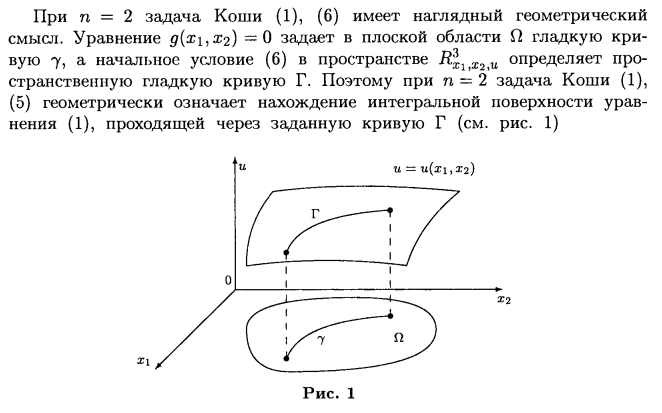
\includegraphics[scale=1.1]{sections/Dima/images/cauchy.png}
\end{center}
\par \Def Всякая точка $M_0 \in \gamma$, для которой
$$\dot{g}(M_0)=(a(M_0), grad \: g(M_0))=0,$$
\par называется характеристической точкой уравнения (\ref{cauchy-first}).

\par \Note Тот факт, что $M_0 \in \gamma$ является характеристической точкой (\ref{cauchy-first}), геометрически означает, что вектор $a(M_0)$ касается поверхности $\gamma$ в точке $M_0$
или, что то же самое, касается характеристик (\ref{cauchy-first}) в точке $M_0$. В частности, положения равновесия характеристической системы (\ref{cauchy-fourth}) и особые точки поверхности $\gamma$ являются характеристическим точками уравнения (\ref{cauchy-first}). Если при $n=2$ кривая $\gamma$ является характеристикой (\ref{cauchy-first}), то каждая точка $\gamma$ является характеристической точкой (\ref{cauchy-first}).

\par \textbf{Теорема 2.} Если $M_0 \in \gamma$ не является характеристической точкой уравнения (\ref{cauchy-first}), то в некоторой окрестности $V \subset \Omega$ точки $M_0$ решение задачи
Коши (\ref{cauchy-first}), (\ref{cauchy-sixth}) существует и единственно.

\par \Proof Так как $M_0$ не характеристическая точка, то $a(M_0) \neq 0$, значит в некоторой окрестности $V$ точки $M_0$ существуют $(n -1)$ независимые в точке $M_0$ первые интегралы $u_l(x), l=1, \ldots, n-1$, характеристической системы (\ref{cauchy-fourth}). По теореме 1 в окрестности $V$ общее
решение (\ref{cauchy-first}) имеет вид
$$u(x)=F[u_1(x), \ldots, u_{n-1}(x)],$$
\par где $F$ — произвольная непрерывно дифференцируемая функция. Покажем, что начальное условие (\ref{cauchy-sixth}) однозначно определяет вид функции $F$. С этой целью в окрестности $V$ рассмотрим систему уравнений
\begin{equation}\label{cauchy-seventh}
    \begin{cases}
      u_l(x)=u_l, l = 1, \ldots, n-1\\
      g(x)=0
    \end{cases}\,.
\end{equation}
\par Покажем, что систему (\ref{cauchy-seventh}) можно однозначно разрешить относительно $x=(x_1, \ldots, x_n)$ в окрестности $V$. Проверим для системы (\ref{cauchy-seventh}) выполнение условий теоремы о системе неявных функций.
\par Все функции в системе (\ref{cauchy-seventh}) непрерывно дифференцируемы в окрестности $V$. Осталось показать, что якобиан
$$\left. \frac{\partial (u_1, \ldots, u_{n-1}, g)}{\partial (x_1, \ldots, x_n)}\right|_{M_0} \neq 0$$
\par Рассуждаем от противного. Пусть якобиан равен нулю. Так как первые $(n-1)$ строк якобиана линейно независимы, то в таком случае последняя его строка линейно зависит от его первых $(n-1)$ строк. Следовательно, найдутся числа $c_l$, $l=1, \ldots, n-1$, одновременно не равные нулю, такие, что
$$\frac{\partial g(M_0)}{\partial x_j}=\sum_{l=1}^{n-1} c_l \frac{\partial u_l(M_0)}{\partial x_j}, \: \forall j = 1, \ldots, n$$
\par Поэтому
$$\dot{g}(M_0)=\sum_{j=1}^n a_j(M_0) \frac{\partial g(M_0)}{\partial x_j}=\sum_{j=1}^n a_j(M_0) \sum_{l=1}^{n-1} c_l \frac{\partial u_l(M_0)}{\partial x_j}=\sum_{l=1}^{n-1} c_l \sum_{j=1}^n a_j(M_0) \frac{\partial u_l(M_0)}{\partial x_j}=\sum_{l=1}^{n-1} c_l \dot{u}_l(M_0)=0$$

\par в силу того, что $u_l(x), l=1, \ldots, n-1$ — первые интегралы (\ref{cauchy-fourth}).

\par С другой стороны, $\dot{g}(M_0) \neq 0$, так как по условию теоремы $M_0 \in \gamma$ не является характеристической точкой (\ref{cauchy-first}). Противоречие. Поэтому в окрестности $V$ выполнены все условия теоремы о неявной функции и система уравнений (\ref{cauchy-seventh}) допускает в окрестности $V$ единственное
непрерывно дифференцируемое решение $x=\omega(u_1, \ldots, u_{n-1})$.

\par Для всех $x \in \gamma \cap V$ функция
$$\varphi(x)=\varphi[\omega(u_1, \ldots, u_{n-1})] \equiv \Phi(u_1, \ldots, u_{n-1})$$
\par является известной непрерывно дифференцируемой функцией $u_1, \ldots, u_{n-1}$. По построению отсюда следует, что
$$u(x)=\Phi[u_1(x), \ldots, u_{n-1}(x)]$$
\par является искомым единственным решением задачи Коши (\ref{cauchy-first}), (\ref{cauchy-sixth}) в окрестности V, так как $u(x)$ — первый интеграл (\ref{cauchy-fourth}) и удовлетворяет начальному условию (\ref{cauchy-sixth}). \EndProof

\newpage

\section{Элементы вариационного исчисления}

\subsection{Основные понятия. Простейшая задача вариационного исчисления. Необходимое условие слабого экстремума}
\setcounter{equation}{0}
\textbf{Определение.}

\textit{Метрическим пространством} называется пара $(X, \rho)$, где 
$X$ -- произвольное непустое множества, а $\rho: X \times X \to \R_+$ -- метрика, которая
удовлетворяет следующим аксиомам:

\begin{enumerate}
    \item $\forall x, y \in X\ \rho(x, y) = 0 \Leftrightarrow x = y$
    \item $\forall x, y \in X\ \rho(x, y) = \rho(y, x)$
    \item $\forall x, y, z \in X\ \rho(x, y) \leqslant \rho(x, z) + \rho(z, y)$
\end{enumerate}

\textbf{Замечание}

В любом нормированном пространстве можно ввести такую метрику:
$\rho(x, y) = \| x - y \|$

\textbf{Нормы для некоторых пространств}

$$
    \left\| f(x) \right\|_{C [a, b]} = \sup_{x \in [a, b]} \left| f(x) \right|
$$

$$
    \left\| f(x) \right\|_{C^k [a, b]} = 
    \sum_{i = 0}^k \max_{x \in [a, b]} \left| f^{(i)} (x) \right|
$$

В частности, норма для $C^1 [a, b]$:

$$
    \left\| f(x) \right\|_{C^1 [a, b]} = 
    \max_{x \in [a, b]} \left| f(x) \right| + 
    \max_{x \in [a, b]} \left| f'(x) \right|
$$

\textbf{Определение.}

Пусть $(X, \rho)$ -- метрическое пространство, $M \subset X$.
Отображение $F: M \to \R$ называется \textit{функционалом}
с облатью определения $M$.

Пусть $F(x, y, p)$ -- непрерывно дифференируемая функция на 
$[a, b] \times \R^2$. Рассмотрим функционал 

\begin{equation}\label{J_func}
    J(y) = \int_a^b F(x, y, y')dx, \;\;y(a) = A,\;\; y(b) = B,
\end{equation}

определённый на множестве 
$M = \{ y(x) \in C^1 [a, b]: y(a) = A, y(b) = B\}$.

\textbf{Определение.}

Функция $\widehat{y}(x) \in M$ называется \textit{слабым локальным минимум (максимумом)}
функционала (\ref{J_func}), если

$$
\exists \varepsilon > 0 : \forall y(x) \in M : 
\left\| y - \widehat{y} \right\|_{C^1 [a, b]} < \varepsilon \; \Rightarrow \;
J(y) \geqslant J(\widehat{y}) \;\;\;\left( J(y) \leqslant J(\widehat{y}) \right)
$$

\textbf{Определение.}

Задача на отыскание слабого локального экстремума функционала (\ref{J_func})
называется \textit{простейшей вариационной задачей} или 
\textit{задачей с закреплёнными концами}.

Рассмотрим две фукнции $y_1(x), y_2(x) \in M$ 
и определим $\eta(x) := y_1(x) - y_2(x)$. Так как концы у функций $y_1(x)$ и
$y_2(x)$ фиксированы, то $\eta(a) = 0$ и $\eta(b) = 0$. Назовём функцию
$\eta$ \textit{вариацией} и введём обозначение для множества 
допустимых вариаций:
$$
    \mathring{C}^1 [a, b] := \{ y(x) \in C^1 [a, b] : y(a) = 0, y(b) = 0\}
$$

Пусть $y(x) \in M, \eta(x) \in \mathring{C}^1 [a, b]$. 
Рассмотрим семейство функций 
$y_{\alpha} (x) = y(x) + \alpha \eta(x), \alpha \in \R$.
Понятно, что для любого $\alpha$ $y_{\alpha}(x) \in M$.
Мы хотим ввести понятие, аналогичное производной по направлению для
числовых функций.

$$
J(y + \alpha \eta) = 
\int_a^b F \left[ x; y(x) + \alpha \eta(x), y'(x) + \alpha \eta'(x) \right]
dx
$$

При фиксированных $y$ и $\eta$ эта функция зависит только от числового
аргумента $\alpha$.
\pagebreak

\textbf{Определение.}

Выражение $\left. \frac{d}{d\alpha} J(y + \alpha \eta) \right|_{\alpha = 0}$
, где $\eta \in \mathring{C}^1 [a, b]$ называется
\textit{первой вариацией функционала $J(y)$ на функции $y(x)$}
и обозначается $\delta J[y, \eta(x)]$.
\bigbreak
\textbf{Теорема.}

Если $\widehat{y}(x) \in M$ является решением простейшей
вариационной задачи, то
$$
\forall \eta(x) \in \mathring{C}^1 [a, b] \ \ 
\delta J \left[ \widehat{y}, \eta(x) \right] = 0
$$

\underline{Доказательство.}

Пусть, без ограничения общности, 
$\widehat{y}$ -- слабый локальный минимум $J(y)$.
Тогда

$$
\exists \varepsilon > 0 : \forall y(x) \in M : 
\left\| y - \widehat{y} \right\|_{C^1 [a, b]} < \varepsilon \ 
J(\widehat{y}) \leqslant J(y)
$$

Зафиксировав $\eta(x)$, подберём 
$\alpha_0 : \| \alpha_0 \eta \|_{C^1} < \varepsilon$.
Тогда 
$\forall \alpha : |\alpha| < \alpha_0 \ \;\| \alpha \eta \| < \varepsilon$.

Рассмотрим числовую функцию 
$\Phi(\alpha) := J(\widehat{y} + \alpha \eta)$.
Так как $\widehat{y}$ -- слабый локальный экстремум $J(y)$, то

$$
\Phi(\alpha) = J(\widehat{y} + \alpha \eta) \geqslant 
J(\widehat{y}) = \Phi(0)
$$

Получается, что функция $\Phi(\alpha)$ имеет минимум в точке
$\alpha = 0$, а значит $\Phi'(0) = 0$.
Это и означает, что 
$
\forall \eta(x) \in \mathring{C}^1 [a, b] \ \ 
\delta J[\widehat{y}, \eta(x)] = 0
$.
\bigbreak
\textbf{Лемма Лагранжа (или основная лемма вариационного исчисления).}


\begin{equation*}
\text{Если } f(x) \in C [a, b] \text{ и } 
\int_a^b f(x) \eta(x) dx = 0 \ \ \forall \eta(x) \in \mathring{C}^1 [a, b],
\text{то } f(x) \equiv 0 \text{ на } [a, b].
\end{equation*}

\underline{Доказательство.}

Предположим, что $f(x) \ \cancel{\equiv}\  0$ на $[a, b]$.
Тогда $\exists x_0 \in (a, b) : f(x_0) \neq 0$ 
(пусть, для определённости, $f(x_0) > 0$).
Так как функция $f$ непрерывна, то 
$\exists \varepsilon > 0 : 
\forall x \in (x_0 - \varepsilon, x_0 + \varepsilon) \subset (a, b) \ f(x) > 0$.

Теперь выберем $\eta(x)$ следующим образом:

\begin{align*}
    \eta(x) = 
    \begin{cases}
        \left( x - (x_0 - \varepsilon) \right)^2
        \left( x - (x_0 + \varepsilon) \right)^2,
        &x \in (x_0 - \varepsilon, x_0 + \varepsilon)\\
        0, & x \notin (x_0 - \varepsilon, x_0 + \varepsilon)
    \end{cases}
\end{align*}

Функция $\eta(x)$ имеет вид "шапочки" на 
$(x_0 - \varepsilon, x_0 + \varepsilon)$ 
и гладким образом спускается к нулю, 
поэтому $\eta(x) \in \mathring{C}^1 [a, b]$.

Так как на $(x_0 - \varepsilon, x_0 + \varepsilon)$ и $f(x) > 0$, 
и $\eta(x) > 0$, то

$$
\int_a^b f(x) \eta(x) dx = 
\int_{x_0 - \varepsilon}^{x_0 + \varepsilon} f(x) \eta(x) dx > 0.
$$

Получилось противоречие с условием
$\int_a^b f(x) \eta(x) dx = 0 \ \ \forall \eta(x) \in \mathring{C}^1 [a, b]$,
а значит $f(x) \equiv 0$ на $[a, b]$.
\bigbreak
\textbf{Теорема (необходимое условие слабого локального экстремума).}

Пусть $F(x; y, p)$ -- дважды непрерывно дифференцируемая функция
$\forall x \in [a, b]$ и $\forall (y, p) \in \R^2$.
Если непрерывно дифференцируемая функция $\widehat{y}$ является
решением простейшей вариационной задачи для (\ref{J_func}), то
эта функция удовлетворяет уравнению Эйлера:

\begin{equation}\label{euler_eq}
\frac{\partial F}{\partial y} 
- \frac{d}{dx} \left( \frac{\partial F}{\partial y'} \right) = 0
\end{equation}

на $[a, b]$.

\pagebreak

\underline{Доказательство.}

Везде далее будем подразумеваться, что все записанные тождества верны для
$y = \widehat{y}$.

Распишем $\delta J(y, \eta(x))$:
\begin{multline*}
\delta J(y, \eta(x)) = 
\left. \frac{d}{d\alpha} J(y + \alpha \eta) \right|_{\alpha = 0} = 
\left. \left[ \frac{d}{d\alpha}
\int_a^b F(x; y + \alpha \eta,  y' + \alpha \eta') dx
\right] \right|_{\alpha = 0} = \\
= \left. \left[ \int_a^b 
\left( 
\frac{\partial F(x, y + \alpha \eta, y' + \alpha \eta')}
{\partial y} \cdot \eta +
\frac{\partial F(x, y + \alpha \eta, y' + \alpha \eta')}
{\partial y'} \cdot \eta' \right) dx
\right] \right|_{\alpha = 0} = \\
= \int_a^b \left(
\frac{\partial F(x, y, y')}
{\partial y} \cdot \eta + 
\frac{\partial F(x, y, y')}{\partial y'} \cdot \eta'
\right) dx
\end{multline*}

Проинтегрируем 
$\int \limits_a^b \frac{\partial F(x, y, y')}
{\partial y'} \cdot \eta' dx$ 
по частям:

\begin{equation*}
\int_a^b \frac{\partial F(x, y, y')}
{\partial y'} \cdot \eta' dx = 
\underbrace{\left. 
\frac{\partial F(x, y, y')}{\partial y'}
\cdot \eta(x) \right|_{x = a}^{x = b}}
_{= 0, \text{ так как } \eta(a) = \eta(b) = 0} 
- \int_a^b \frac{d}{dx} \left(
\frac{\partial F(x, y, y')}{\partial y'}
\right) \cdot \eta(x) dx
\end{equation*}

\begin{equation*}
\delta J(y, \eta(x)) = 
\int_a^b \left(
\frac{\partial F(x, y, y')}{\partial y} -
\frac{d}{dx} \left(
\frac{\partial F(x, y, y')}{\partial y'}
\right)
\right) \cdot \eta(x) dx
\end{equation*}

Так как $y$ -- локальный экстремум, то по предыдущей теореме
$\forall \eta(x) \in \mathring{C}^1 [a, b] \ \ 
\delta J(y, \eta(x)) = 0$:

$$
\forall \eta(x) \in \mathring{C}^1 [a, b] \ \ 
\int_a^b \left(
\frac{\partial F(x, y, y')}
{\partial y} -
\frac{d}{dx} \left(
\frac{\partial F(x, y, y')}{\partial y'}
\right)
\right) \cdot \eta(x) dx = 0
$$

Теперь по лемме Лагранжа получаем требуемое:

$$
\frac{\partial F(x, y, y')}
{\partial y} -
\frac{d}{dx} \left(
\frac{\partial F(x, y, y')}{\partial y'}
\right) = 0
$$

на $[a, b]$.

\textbf{Определение.}

Решение уравнения (\ref{euler_eq}) называется \textit{экстремалью}
функционала (\ref{J_func}).
Если экстремаль удовлетворяет условиям $y(a) = A, y(b) = B$, то
она называется \textit{допустимой}.
\newpage

\subsection{Задача со свободными концами, необходимое условие слабого экстремума}
Рассмотрим функционал 

\begin{equation}\label{J_func_free}
J(y) = \int_a^b F \left( x; y(x), y'(x)) \right) dx,
\end{equation}
\\
определённый на множестве
$M = \{ y(x) \in C^1 [a, b] : y(a) = A\}$, где
$F \left( x; y, p \right)$ -- дважды непрерывно дифференцируемая
функция на $[a, b] \times \R^2$.
Задача отличается от простейшей вариационной задачи только тем,
что один из концов (в данном случае $b$) не зафиксирован.

\textbf{Определение.}

Задача нахождения слабого локального экстремума функционала
(\ref{J_func_free}) называется
\textit{задачей со свободным концом}.

\textbf{Теорема.}

Если дважды непрерывно дифференцируемая функция 
$\widehat{y}(x) \in M$ даёт слабый локальный экстремум функционала
(\ref{J_func_free}), то на $[a, b]$ $\widehat{y}(x)$ удовлетворяет
уравнению Эйлера

\begin{equation}\label{euler_eq_free}
\frac{\partial F}{\partial y} - \frac{d}{dx} \left(
\frac{\partial F}{\partial y'} \right) = 0
\end{equation}

и при $x = b$:

\begin{equation}\label{extra_cond}
\left. 
\frac{\partial F}{\partial y'} 
\left[ x; \widehat{y}(x), \widehat{y}'(x) \right]
\right|_{x = b} = 0
\end{equation}

\underline{Доказательство.}

Рассмотрим произвольное допустимое приращение 
$\eta(x) \in C^1 [a, b] : \eta(a) = 0$.

Пусть $\Phi(\alpha) = J(\widehat{y} + \alpha \eta), \alpha \in \R$ -- 
непрерывно дифференицруемая функция аргумента $\alpha$;
при $\alpha = 0$ $\Phi(\alpha)$ имеет экстремум.
Следовательно, (в последнем = меняем местами диф-ние и инт-ние)

$$
0 = \Phi'(0) = \left. \frac{d}{d\alpha} 
J( \widehat{y} + \alpha \eta) \right|_{\alpha = 0} = 
\left. \frac{d}{d\alpha} \int_a^b F \left( x, \widehat{y} + \alpha \eta, 
\widehat{y}' + \alpha \eta' \right) dx \right|_{\alpha = 0} = 
\left. \int_a^b \left[
\frac{\partial F}{\partial y} \eta(x) + 
\frac{\partial F}{\partial y'} \eta'(x)
\right] \right|_{y = \widehat{y}(x)} dx
$$

Проинтегрируем второе слагаемое по частям:

$$
\left. \int_a^b \frac{\partial F}{\partial y'} \eta' 
\right|_{y = \widehat{y}} dx = 
\left. \frac{\partial F(x; \widehat{y}, \widehat{y}')}{\partial y'} 
\right|_{x = b} \cdot \eta(b) - 
\left. \int_a^b \frac{d}{dx} \left(
\frac{\partial F}{\partial y'}
\right) \right|_{y = \widehat{y}} \eta(x) dx
$$

Тогда $\Phi'(0)$ запишется следующим образом:

$$
\Phi'(0) = \left. 
\frac{\partial F(x; \widehat{y}, \widehat{y}')}{\partial y'}
\right|_{x = b} \eta(b) + \left. \int_a^b \left[
\frac{\partial F}{\partial y} - 
\frac{d}{dx} \left( \frac{\partial F}{\partial y'} \right) 
\right] \right|_{y = \widehat{y}} \eta(x) dx = 0
$$

Это выполняется для любого $\eta(x) \in C^1 [a, b] : \eta(a) = 0$.
Это, в частности, означает, что это верно для 
$\eta_1(x) \in C^1 [a, b] : \eta(a) = 0, \eta(b) = 0$. При подставлении
$\eta_1(x)$ получаем, что 

$$
\int_a^b \left[
\frac{\partial F}{\partial y} - 
\frac{d}{dx} \left( \frac{\partial F}{\partial y'} \right) 
\right] \eta(x) dx = 0
$$

Используя основную лемму вариационного исчисления, получим условие 
(\ref{euler_eq_free}). Это означает, что второе слагаемое в выражении 
$\Phi'(0)$ всегда равно нулю. Получаем, что для всех
$\eta(x) \in C^1 [a, b] : \eta(a) = 0$

$$
\Phi'(0) = \left. 
\frac{\partial F(x; \widehat{y}, \widehat{y}')}{\partial y'}
\right|_{x = b} \eta(b) = 0
$$

Так как можно подобрать вариацию, такую что $\eta(b) \neq 0$, то 
необходимым условием слабого локального экстремума является 
условие (\ref{extra_cond}).
\pagebreak

\textbf{Определение.}

Решение уравнения (\ref{euler_eq_free}) называется
\textit{экстремалью задачи со свободным концом}.
Решение уравнения (\ref{euler_eq_free}), которое удовлетворяет
условию $y(a) = A$ и условию (\ref{extra_cond}), называется
\textit{допустимой экстремалью}.

Для задачи, где не закреплены оба конца, можно получить 
аналогичное необходимое условие слабого локального экстремума:

\textbf{Теорема.}

Рассмотрим функционал 

\begin{equation*}
J(y) = \int_a^b F \left( x; y(x), y'(x)) \right) dx,
\end{equation*}
\\
где $y(x) \in C^1 [a, b]$ (то есть оба конца не закреплены) и
$F \left( x; y, p \right)$ -- дважды непрерывно дифференцируемая
функция на $[a, b] \times \R^2$.

Если $\widehat{y}(x) \in C^1 [a, b]$ даёт слабый локальный экстремум
функционала $J(y)$, то $\widehat{y}(x)$ удовлетворяет
следующим условиям:

$$
\frac{\partial F}{\partial y} - 
\frac{d}{dx} \left( \frac{\partial F}{\partial y'} \right) = 0
$$

$$
\left. \frac{\partial F}{\partial y'} \right|_{x = a} = 
\left. \frac{\partial F}{\partial y'} \right|_{x = b} = 0
$$
\newpage

\subsection{Задача для функционалов, зависящих от нескольких неизвестных функций, задача для функционалов, содержащих производные высших порядков}
\textbf{Замечание.}

Функционалы, зависящие от нескольких неизвестных функций, можно
интерпретировать как функционалы, зависящие от вектор-функции.

Пусть $C_n^1 [a, b]$ -- множество непрерывно дифференцируемых
вектор-функций с компонентами \\
$y_1(x), \dots, y_n(x)$, определёнными на
множестве $[a, b]$. Норма на этом пространстве вводится следующим образом:

$$
\left\| \Vec{y}(x) \right\|_{C_n^1 [a, b]} = 
\max_{x \in [a, b]} |y(x)| + \max_{x \in [a, b]} |y'(x)|
$$

Тогда соответствующая метрика определяется как
$\rho(\Vec{y}, \Vec{z}) = \| \Vec{y} - \Vec{z} \|$.

Функционалы для вектор-функций определяются аналогично:

\begin{equation}\label{J_func_vec}
J(\Vec{y}) = \int_a^b F \left[ x; \Vec{y}(x), \Vec{y'}(x) \right] dx,
\end{equation}

где $F \left[ x; \Vec{y}(x), \Vec{y'}(x) \right]$ --
дважды непрерывно дифференцируемая функция на $[a, b] \times \R^{2n}$.

В качестве аргументов функции $J(\Vec{y})$ будем
рассматривать вектор-функции из множества 
$M = \left\{ \Vec{y}(x) \in C_n^1 [a, b] : 
\Vec{y}(a) = \Vec{A}, \Vec{y}(b) = \Vec{B} \right\}$.

\textbf{Определение.}

Функция $\widehat{y}(x) \in M$ называется 
\textit{слабым локальным минимумом (максимумом)} 
функционала (\ref{J_func_vec}), если

$$
\exists \varepsilon > 0 : \forall \Vec{y} \in M :
\left\| \widehat{\Vec{y}} - \Vec{y} \right\|_{C_n^1} < \varepsilon
\ \ J(\Vec{y}) \geqslant J (\widehat{\Vec{y}})
\ \left( J(\Vec{y}) \leqslant J (\widehat{\Vec{y}}) \right)
$$

\textbf{Теорема.}

Если дважды непрерывно дифференцируемая вектор-функция 
$\widehat{\Vec{y}} \in M$ даёт слабый локальный экстремум
функционала (\ref{J_func_vec}), то $\widehat{\Vec{y}}$
удовлетворяет на $[a, b]$ системе уравнений Эйлера:

\begin{equation}
\frac{\partial F}{\partial y_i} 
- \frac{d}{dx} \left( \frac{\partial F}{\partial y_i'} \right) = 0,
\ i = \overline{1, \dots, n}
\end{equation}

\underline{Доказательство.}

Пусть $\widehat{\Vec{y}} = 
\left( y_1(x), \widehat{y_2}(x), \dots, \widehat{y_n}(x) \right)$ --
первая координата свободная, а остальные зафиксируем.
Тогда $J(\Vec{y}) = \widetilde{J}(y_1)$ -- функционал, зависящий от
одной переменной. Это является простейшей вариационной задачей,
экстремум достигается при $\widehat{y_1}(x)$, и необходимым условием
является уравнение Эйлера:

$$
\frac{\partial F}{\partial y_1} 
- \frac{d}{dx} \left( \frac{\partial F}{\partial y_1'} \right) = 0,
$$

Повторив эти действия для каждой координаты, получаем нужную систему.
\bigbreak
\textbf{Функционалы, зависящие от производных высших порядков.}

В этом разделе мы будем работать с функциями из пространства
$C^k [a, b]$. На этом пространстве норму можно ввести следующим образом:

$$
\left\| y \right\|_{C^k [a, b]} = 
\max_{x \in [a, b]} |y(x)| + 
\sum_{i = 1}^k \max_{x \in [a, b]} |y^{(i)}(x)|
$$

Соответствующая метрика вводится следующим образом:
$\rho(y, z) = \| y - z \|_{C^k}$.

Аналогично простейшей вариационной задаче 
введём множество допустимых вариаций:

$$
\mathring{C}^k [a, b] = 
\left\{ y \in C^k [a, b] : y^{(i)}(a) = y^{(i)}(b) = 0, 
i = \overline{0, \dots, k - 1} \right\}
$$
\pagebreak

\textbf{Лемма}

$$
\text{Если } f(x) \in C [a, b] \text{ и } 
\forall \eta \in \mathring{C}^k [a, b]
\int_a^b f(x) \eta(x) dx = 0 \text{, то }
f(x) \equiv 0 \text{ на } [a, b].
$$

\underline{Доказательство.}

Предположим, что $f(x) \not \equiv 0$ на $[a, b]$.
Тогда $\exists x_0 \in (a, b) : f(x_0) \neq 0$ (пусть,
без ограничения общности, $f(x_0) > 0$).
Так как $f(x)$ непрерывна, то 
$\exists \varepsilon > 0 : 
\left( x - (x_0 - \varepsilon) \right)^{2k} \subset (a, b)$ и
и $f(x) > 0 \forall x \in (x_0 - \varepsilon, x_0 + \varepsilon)$.
Подберём такую вариацию:

\begin{equation*}
\eta(x) = 
\begin{cases}
\left( x - (x_0 - \varepsilon) \right)^{2k}
\left( x - (x_0 + \varepsilon) \right)^{2k},
x \in (x_0 - \varepsilon, x_0 + \varepsilon)
\\
0, \text{ иначе}
\end{cases}
\end{equation*}

Можно проверить, что $\eta(x) \in \mathring{C}^k [a, b]$.
Поэтому 

\begin{equation*}
0 = \int_a^b f(x) \eta(x) dx =
\int_{x_0 - \varepsilon}^{x_0 + \varepsilon} f(x) \eta(x) dx > 0
\end{equation*}

Получили противоречие. Получается, что $f(x) \equiv 0$ на $[a, b]$.

\textbf{Определение.}

Рассмотрим функционал

\begin{equation}\label{J_func_der}
J(y) = \int_a^b F \left[ x; y(x), \dots, y^{(k)}(x) \right] dx,
\end{equation}

определённый на множестве
$M = \{ y(x) \in C^k [a, b] : y^{(i)}(a) = A_i, y^{(i)}(b) = B_i, 
i = \overline{1, \dots, k - 1} \}$,\\
где $F \left[ x; y(x), \dots, y^{(k)}(x) \right]$ -- $(k + 1)$ раз
непрерывно дифференцируемая функция.

Скажем, что $\widehat{y} \in M$ даёт 
\textit{слабый локальный минимум (максимум)} 
функционала (\ref{J_func_der}), если

$$
\exists \varepsilon > 0 : \forall y(x) \in M : 
\| \widehat{y} - y\|_{C^k} < \varepsilon \ \ 
J(y) \geqslant J(\widehat{y}) \left( J(y) \leqslant J(\widehat{y}) \right).
$$

Пусть $y(x) \in M$ и $\eta(x) \in \mathring{C}^k [a, b]$.
При фиксированных $y(x)$ и $\eta(x)$ определим $\Phi(\alpha), \alpha \in \R$:

$$
\Phi(\alpha) = J( y(x) + \alpha \eta(x) ) = 
\int_a^b F \left( x; y + \alpha \eta, \dots, 
y^{(k)} + \alpha \eta^{(k)} \right) dx
$$

Аналогично простейшей вариационной задаче,
если $\widehat{y}$ даёт экстремум $J(y)$, 
то $\Phi(\alpha)$ имеет экстремум при $\alpha = 0$:

$$
\Phi'(0) = \left. \frac{dJ(\widehat{y} + \alpha \eta)}{d\alpha} 
\right|_{\alpha = 0} = 
\int_a^b \left[ 
\frac{\partial F}{\partial \widehat{y}} \eta(x) + 
\frac{\partial F}{\partial \widehat{y}'} \eta'(x) + \dots + 
\frac{\partial F}{\partial \widehat{y}^{(k)}} \eta^{(k)}(x)
\right] dx
$$

\textbf{Определение.}
\\
Выражение $\Phi'(0)$, где $\eta(x) \in \mathring{C}^k [a, b]$, называется
\textit{первой вариацией функционала (\ref{J_func_der})} \\
и обозначается $\delta J[y; \eta]$.

\textbf{Теорема (необходимое условие слабого локального экстремума).}

Пусть $\widehat{y} \in M$ является $2k$ дифференцируемой функцией и 
даёт слабый локальный экстремум функционала (\ref{J_func_der}).
Тогда на $[a, b]$ $\widehat{y}(x)$ удовлетворяет 
уравнению Эйлера-Пуассона:

\begin{equation}\label{euler_pois_eq}
\frac{\partial F}{\partial y} - 
\frac{d}{dx} \left( \frac{\partial F}{\partial y'} \right) +
\frac{d^2}{dx^2} \left( \frac{\partial F}{\partial y''} \right) - \dots
+ (-1)^k 
\frac{d^k}{dx^k} \left( \frac{\partial F}{\partial y^{(k)}} \right) = 0
\end{equation}

\underline{Доказательство.}

Так как $\widehat{y}$ даёт слабый локальный экстремум, то
$\delta J [\widehat{y}, \eta(x)] = 0 \ \ 
\forall \eta(x) \in \mathring{C}^k [a, b]$. Распишем $\delta J$:

$$
0 = \delta J [\widehat{y}, \eta(x)] = 
\int_a^b \left[ 
\frac{\partial F}{\partial \widehat{y}} \eta(x) + 
\frac{\partial F}{\partial \widehat{y}'} \eta'(x) + \dots + 
\frac{\partial F}{\partial \widehat{y}^{(k)}} \eta^{(k)}(x)
\right] dx
$$
\pagebreak

Проинтегрируем по частям каждое слагаемое в этой формуле 
столько раз, сколько нужно, чтобы избавиться от всех производных $\eta(x)$.
Например, для $i$-го слагаемого поступим следующим образом:

\begin{multline*}
\int_a^b \frac{\partial F}{\partial y^{(i)}} \eta^{(i)} dx = 
\int_a^b \frac{\partial F}{\partial y^{(i)}} d\eta^{(i - 1)} = 
\underbrace{\left. \frac{\partial F}{\partial y^{(i)}} \eta^{(i - 1)} 
\right|_a^b}_{= 0 \text{, так как } 
\eta^{(i - 1)}(a) = \eta^{(i - 1)}(b) = 0} - 
\int_a^b \frac{d}{dx} \left( \frac{\partial F}{\partial y^{(i)}} \right)
\eta^{(i - 1)} dx = \\
= - \left[ 
\underbrace{\left. \frac{d}{dx} \left( 
\frac{\partial F}{\partial y^{(i)}} \right) 
\eta^{(i - 2)} \right|_a^b}_{ = 0} - 
\int_a^b \frac{d^2}{dx^2} \left( 
\frac{\partial F}{\partial y^{(i)}} \right) \eta^{(i - 2)} dx
\right] = 
\int_a^b \frac{d^2}{dx^2} \left( \frac{\partial F}{\partial y^{(i)}}
\right) \eta^{(i - 2)} dx = \dots
\end{multline*}

Для последнего слагаемого получится так:

$$
\int_a^b \frac{\partial F}{\partial y^{(k)}} \eta^{(k)} dx = 
(-1)^k \int_a^b \frac{d^k}{dx^k} \left( 
\frac{\partial F}{\partial y^{(k)}} \right) \eta(x) dx
$$

Тогда первая вариация перепишется в следующем виде:

$$
0 = \delta J [\widehat{y}, \eta(x)] = 
\int_a^b \left[ 
\frac{\partial F}{\partial y} - 
\frac{d}{dx} \left( \frac{\partial F}{\partial y'} \right) + \dots + 
(-1)^k \frac{d^k}{dx^k} \left( \frac{\partial F}{\partial y^{(k)}} \right)
\right] \eta(x) dx \ \ 
\forall \eta(x) \in \mathring{C}^k [a, b]
$$

Используя доказанную лемму, получаем необходимое уравнение.

\newpage

\subsection{Изопериметричеcкая задача}
Пусть функции $F(x; y, p)$ и $G(x; y, p)$ дважды непрерывно
дифференцируемы на $[a, b] \times \R^2$. Рассмотрим функционал

\begin{equation}\label{J_func_isoper}
J(y) = \int_a^b F(x; y, y') dx,
\end{equation}

определённый на множестве ($A, B, l$ -- фиксированные числа)
$$
M = \left\{ y \in C^1 [a, b] : y(a) = A, y(b) = B, 
K(y) = \int_a^b G(x; y, y') dx = l \right\}
$$

Условие $K(y) = l$ называют \textit{условием связи}.

\textbf{Определение.}

Функция $\widehat{y}(x) \in M$ называется называется 
\textit{слабым локальным минимумом (максимумом)} функционала 
(\ref{J_func_isoper}), если 

$$
\exists \varepsilon > 0 : \forall y \in M : 
\| y - \widehat{y} \|_{C^1 [a, b]} < \varepsilon \ \ 
J(y) \geqslant J(\widehat{y}) 
\left( J(y) \leqslant J(\widehat{y}) \right)
$$

\textbf{Определение.}

\textit{Изопериметрической задачей} называется задача нахождения
слабого локального экстремума функционала (\ref{J_func_isoper}).

\textbf{Замечание.}

Изопериметрическая задача похожа на задачу поиска
условного экстремума числовых функций.

Так же, как и для условного экстремума числовых функций,
определим лагранжиан:

$$
L(x, y; \lambda) = F(x, y, y') + \lambda G(x, y, y'), \lambda \in \R
$$

$\lambda$ называется \textit{множителем Лагранжа}.

Также при формулировке необходимого условия потребуем, чтобы 

$$
\delta K(y, \eta) = \int_a^b \left(
\frac{\partial G}{\partial y} \eta(x) + 
\frac{\partial G}{\partial y'} \eta'(x)
\right) dx \ \ \forall \eta \in \mathring{C}^1 [a, b]
$$
\\
не равнялась тождественному нулю, так как иначе 
экстремум функционала может равняться $l$, а значит
условию связи будет удовлетворять только одна функция, и 
изопериметрическая задача будет несодержательной.

\textbf{Теорема (необходимое условие).}

Пусть дважды непрерывно дифференцируемая функция $\widehat{y}(x) \in M$
является решением изопериметрической задачи и пусть
$\delta K (\widehat{y}, \eta) \not \equiv 0$ для всех 
$\eta \in \mathring{C}^1 [a, b]$.
Тогда найдётся такое значение $\lambda \in \R$, что на $[a, b]$
функция $\widehat{y}$ будет удовлетворять уравнению Эйлера

\begin{equation}\label{euler_eq_isoper}
\frac{\partial L}{\partial y} - \frac{d}{dx} \left(
\frac{\partial L}{\partial y'} \right) = 0
\end{equation}

\underline{Доказательство.}

Из условия теоремы следует, что $\exists \eta_0(x) \in \mathring{C}^1 [a, b]$
такая, что $\delta K [ \widehat{y}, \eta_0(x) ] \neq 0$.

Рассмотрим следующие функции:

$$
u = \varphi(\alpha, \beta) = 
J [\widehat{y}(x) + \alpha \eta(x) + \beta \eta_0(x)],
\alpha, \beta \in \R
$$

$$
v = \psi(\alpha, \beta) = 
K [\widehat{y}(x) + \alpha \eta(x) + \beta \eta_0(x)],
\alpha, \beta \in \R
$$

Используя теоремы о непрерывности и дифференцируемости собственных
интегралов, зависящих от параметра, получаем:

$$
\varphi(0, 0) = J(\widehat{y}), \ \ 
\frac{\partial \varphi (0, 0)}{\partial \alpha} = 
\delta J[ \widehat{y}(x), \eta(x)], \ \ 
\frac{\partial \varphi (0, 0)}{\partial \beta} = 
\delta J[ \widehat{y}(x), \eta_0(x)]
$$

$$
\psi(0, 0) = K(\widehat{y}), \ \ 
\frac{\partial \psi (0, 0)}{\partial \alpha} = 
\delta K[ \widehat{y}(x), \eta(x)], \ \ 
\frac{\partial \psi (0, 0)}{\partial \beta} = 
\delta K[ \widehat{y}(x), \eta_0(x)]
$$

Далее можно расписать все первые вариации подобным образом:

$$
\delta J [\widehat{y}, \eta(x)] = 
\int_a^b \left[ 
\left. \frac{\partial F}{\partial y} \right|_{y = \widehat{y}(x)} \eta(x) +
\left. \frac{\partial F}{\partial y'} \right|_{y = \widehat{y}(x)} \eta'(x)
\right] dx
$$

Покажем, что якобиан

$$
\frac{\partial (\varphi, \psi)}{\partial (\alpha, \beta)} \equiv 0
\ \ \forall \eta(x) \in \mathring{C}^1 [a, b]
$$

Предположим, что $\exists \eta_1(x) \in \mathring{C}^1 [a, b]$ такое, что
$\frac{\partial (\varphi, \psi)}{\partial (\alpha, \beta)} \neq 0$.
Это означает, что существует окрестность точки $(0, 0)$,
в которой система

\begin{equation*}
\begin{cases}
u = \varphi(\alpha, \beta) \\
v = \psi(\alpha, \beta)
\end{cases}
\end{equation*}

разрешима относительно $\alpha$ и $\beta$.

Пусть, без ограничения общности, $\widehat{y}$ даёт минимум
функционала (\ref{J_func_isoper}). Тогда рассмотрим такую систему:

\begin{equation*}
\begin{cases}
\varphi(\alpha, \beta) = \varphi(0, 0) - \varepsilon,\  \varepsilon > 0 \\
\psi(\alpha, \beta) = \psi(0, 0)
\end{cases}
\end{equation*}

По доказанному, решение этой системы существует и единственно --
обозначим его $(\widehat{\alpha}, \widehat{\beta})$. Тогда у нас выполнено

$$
\varphi(\widehat{\alpha}, \widehat{\beta}) = \varphi(0, 0) - \varepsilon = 
J(\widehat{y}) - \varepsilon, \ \ 
\psi(\widehat{\alpha}, \widehat{\beta}) = \psi(0, 0) = 
K(\widehat{y}) = l
$$

Это значит, что существует функция 
($\widehat{y}(x) + \widehat{\alpha} \eta_1(x) + \widehat{\beta} \eta_0(x)$)
такая, что

$$
J(\widehat{y}(x) + \widehat{\alpha} \eta_1(x) + \widehat{\beta} \eta_0(x)) =
J(\widehat{y}) - \varepsilon < J(\widehat{y}), \ \ 
K(\widehat{y}(x) + \widehat{\alpha} \eta_1(x) + \widehat{\beta} \eta_0(x)) =
l
$$

Это противоречит тому, что $\widehat{y}$ даёт слабый локальный минимум.
Таким образом, мы доказали, что 

$$
\frac{\partial (\varphi, \psi)}{\partial (\alpha, \beta)} \equiv 0
\ \ \forall \eta(x) \in \mathring{C}^1 [a, b]
$$

Распишем этот якобиан:

$$
\left. \frac{\partial (\varphi, \psi)}{\partial (\alpha, \beta)}
\right|_{\alpha = \beta = 0} = 
\begin{vmatrix}
\delta J(\widehat{y}, \eta) & \delta K(\widehat{y}, \eta) \\
\delta J(\widehat{y}, \eta_0) & \delta K(\widehat{y}, \eta_0)
\end{vmatrix}
\equiv 0 \ \ \forall \eta(x) \in \mathring{C}^1 [a, b]
$$

Положим $\lambda = -\frac{\delta J(\widehat{y}, \eta_0)}
{\delta K(\widehat{y}, \eta_0)}$ (здесь мы пользуемся тем, что
$\delta K(\widehat{y}, \eta_0) \neq 0$). Тогда мы получаем, что


$$
\delta J(\widehat{y}, \eta) + \lambda
\delta K(\widehat{y}, \eta) \equiv 0\ \ 
\forall \eta(x) \in \mathring{C}^1 [a, b]
$$

Расписав первые вариации, получаем:

\begin{multline*}
\delta J(\widehat{y}, \eta) + \lambda \delta K(\widehat{y}, \eta) = 
\int_a^b \left. \left( \frac{\partial F}{\partial y} \eta + 
\frac{\partial F}{\partial y'} \eta' \right) 
\right|_{y = \widehat{y}} dx + \lambda
\int_a^b \left. \left( \frac{\partial G}{\partial y} \eta + 
\frac{\partial G}{\partial y'} \eta' \right) \right|_{y = \widehat{y}} dx =
\\ =
\int_a^b \left. \left[
\left( 
\frac{\partial F}{\partial y} + \lambda \frac{\partial G}{\partial y}
\right) \eta(x) + 
\left( 
\frac{\partial F}{\partial y'} + \lambda \frac{\partial G}{\partial y'}
\right) \eta'(x)
\right] \right|_{y = \widehat{y}} dx = 0
\end{multline*}

Проинтегрируем слагаемое с $\eta'(x)$ по частям:

$$
\int_a^b \left( 
\frac{\partial F}{\partial y'} + \lambda
\frac{\partial G}{\partial y'}
\right) d \eta = 
\underbrace{\left. \left( \frac{\partial F}{\partial y'} + \lambda
\frac{\partial G}{\partial y'} \right) \eta \right|_a^b}
_{= 0, \text{ так как } \eta(a) = \eta(b) = 0} - 
\int_a^b \frac{d}{dx} \left(
\frac{\partial F}{\partial y'} + \lambda
\frac{\partial G}{\partial y'}
\right) \eta dx
$$

Воспользовавшись тем, что 
$\frac{\partial L}{\partial y} = \frac{\partial F}{\partial y} + \lambda
\frac{\partial G}{\partial y}$ и 
$\frac{\partial L}{\partial y'} = \frac{\partial F}{\partial y'} + \lambda
\frac{\partial G}{\partial y'}$, получаем:

$$
\int_a^b \left( \frac{\partial L}{\partial y} - \frac{d}{dx}
\left( \frac{\partial L}{\partial y'} \right)
\right) \eta(x) dx = 0 \ \ 
\forall \eta(x) \in \mathring{C}^1 [a, b]
$$

Используя основную лемму вариационного исчисления, получаем
уравнение (\ref{euler_eq_isoper}).

